\documentclass[12pt, twoside]{report}
\usepackage{layout}
\usepackage[utf8]{inputenc}
\usepackage{graphicx}
\usepackage{amsmath}
% \usepackage{fontspec}
\usepackage[a4paper, width=150mm, top=25mm, bottom=25mm, left = 4.0132cm, right = 25mm]{geometry}

\usepackage{setspace}
\usepackage{titlesec}
\usepackage{svg}
\usepackage{float}

\usepackage{multirow}


\graphicspath{ {./src/} }
\titleformat{\chapter}{\Huge\bfseries}{Chapter \thechapter{}.\ }{0ex}{}
\titlespacing*{\chapter}{0 pt}{-\baselineskip}{8 pt}

\onehalfspacing


\begin{document}
% new section with size 24


\chapter{Instrumented arm skateboard (ArmBo)}

\section{ArmBo}

The instrumented arm skateboard (ArmBo) is a platform that consists of three
omnidirectional wheels and an arm-support on top.
It has two sensing modalities: optical encoders at the three omni-directional wheels,
and an inertial measurement unit (IMU).
These sensing modalities can be used to estimate the position and orientation of ArmBo.
The platform is equipped with a Teensy 4.0 microcontroller that acquires
real-time data from the optical encoders and the IMU.
The data is wirelessly streamed to a PC through an HC-05 Bluetooth module as shown in Fig \ref{fig:omniwheel}.
\begin{figure}[hbt!]
    \centering
    \includegraphics[width=\textwidth]{m_omniwheel.png}
    \caption{ArmBo with omni directional wheels and ArUco marker}
    {a) omnidirectional wheel, b) Skematic of ArmBo's coordinate frame, c)
        ArmBo with ArUco marker}
    \label{fig:omniwheel}
\end{figure}


\subsection{Omnidirectional wheels}

The ArmBo is equipped with 3 omni directional wheels as shown in the Fig \ref{fig:omniwheel} a,
the advent of having an omni wheel is that it can slide in any direction,
if we arrange it in a pattern, we can drive the kinematic of the skateboard.
These Omni wheels are attached to optical encoders which can give out relative
angular displacement.

\subsection{ArUco marker}

An ArUco marker is a square-shaped marker that has a wide black border
and an inner binary matrix that determines its identifier as shown in Fig \ref{fig:aruco_intro}.
ArUco markers are commonly used in computer vision applications such as robot
navigation and augmented reality. The ArUco marker has fixed dimensions which
helps the program to estimate its position and orientation, in a real-world frame.
\begin{figure}[hbt!]
    \centering
    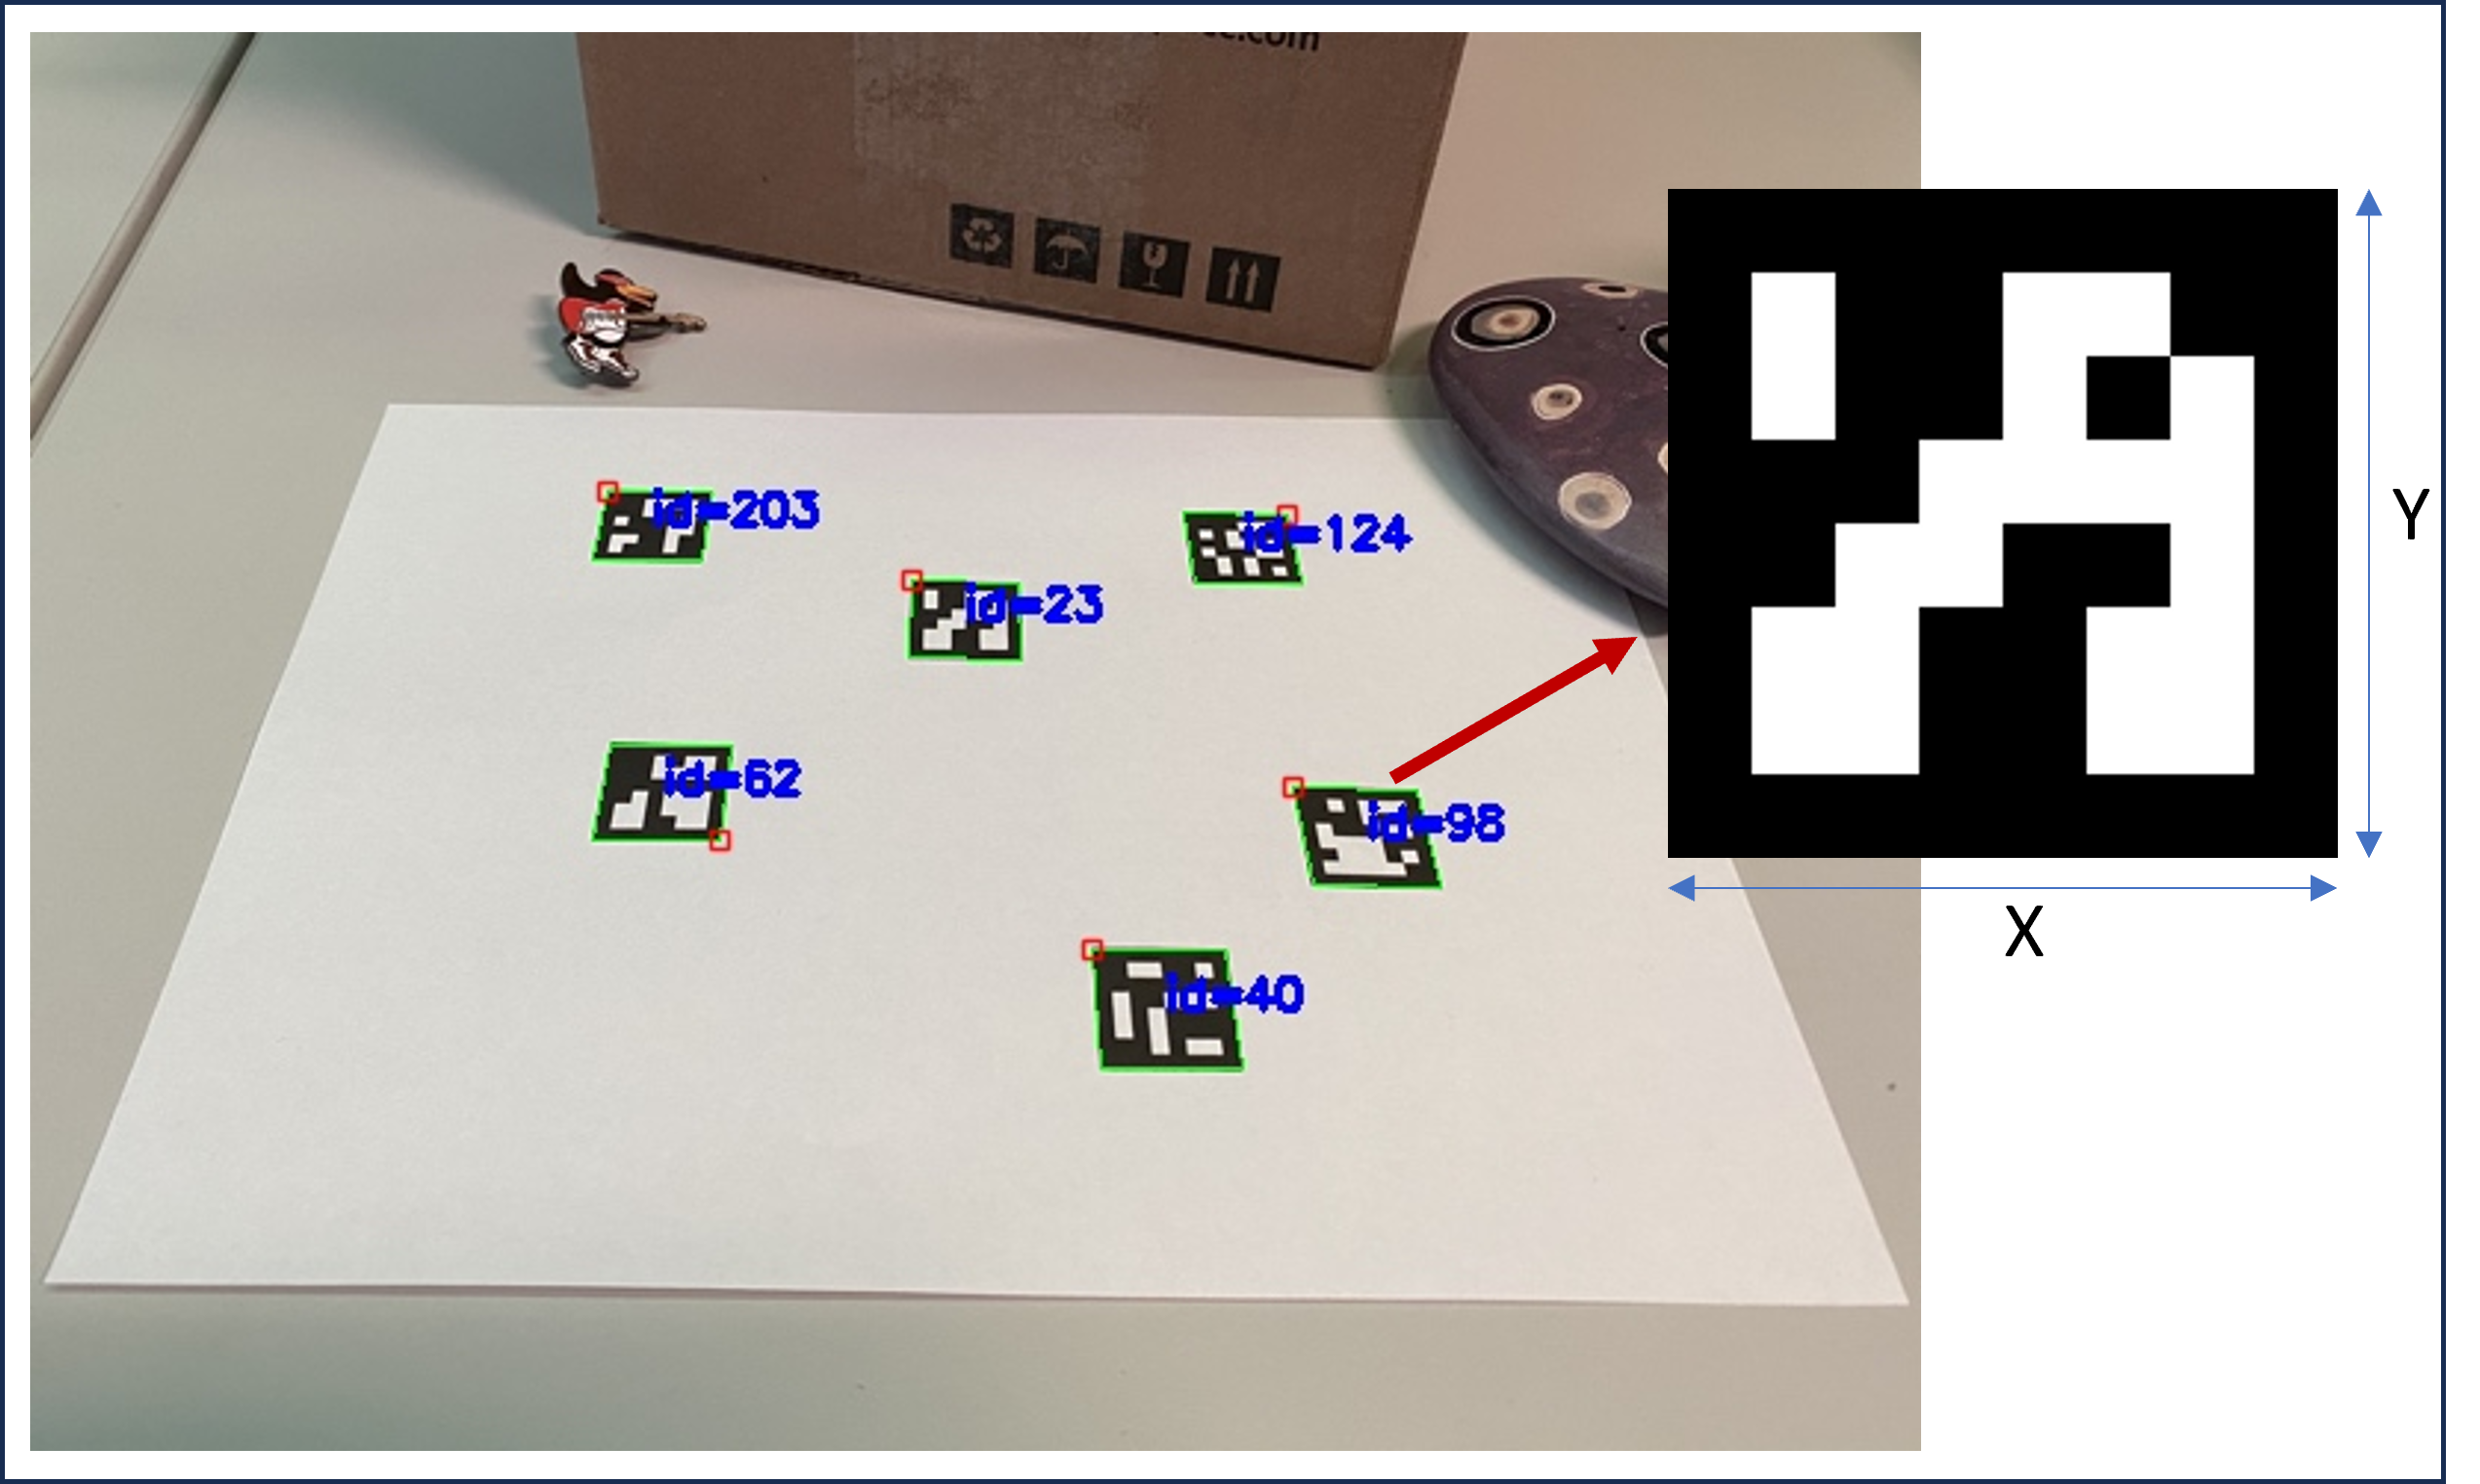
\includegraphics[width=\textwidth]{m_aruco_intro.png}
    \caption{ArUco marker}
    {The figure shows detection of multiple ArUco marker on table, each with unique ID}
    \label{fig:aruco_intro}
\end{figure}

\subsection{Microcontroller and communication protocol}

Teensy 4.0 microcontroller is used to read from the three encoders and an IMU,
and transmit them to PC using a HC-05 bluetooth serial communication protocol. The sampling frequency of
the sensors are set to 100 Hz. The data communication protocol has been customised to ensure
no loss of receiving packets from the controller as shown in Fig \ref{fig:jedi}. \\

The communication starts with two start bytes 0xff, 0xff, followed by 41 bytes of data, finally
ending with check sum byte, which is the sum of all the 41 bytes. The PC receives the data, and
checks the check sum byte, if the check sum byte is correct, the data is processed, else the data is discarded.


\begin{figure}[hbt!]
    \centering
    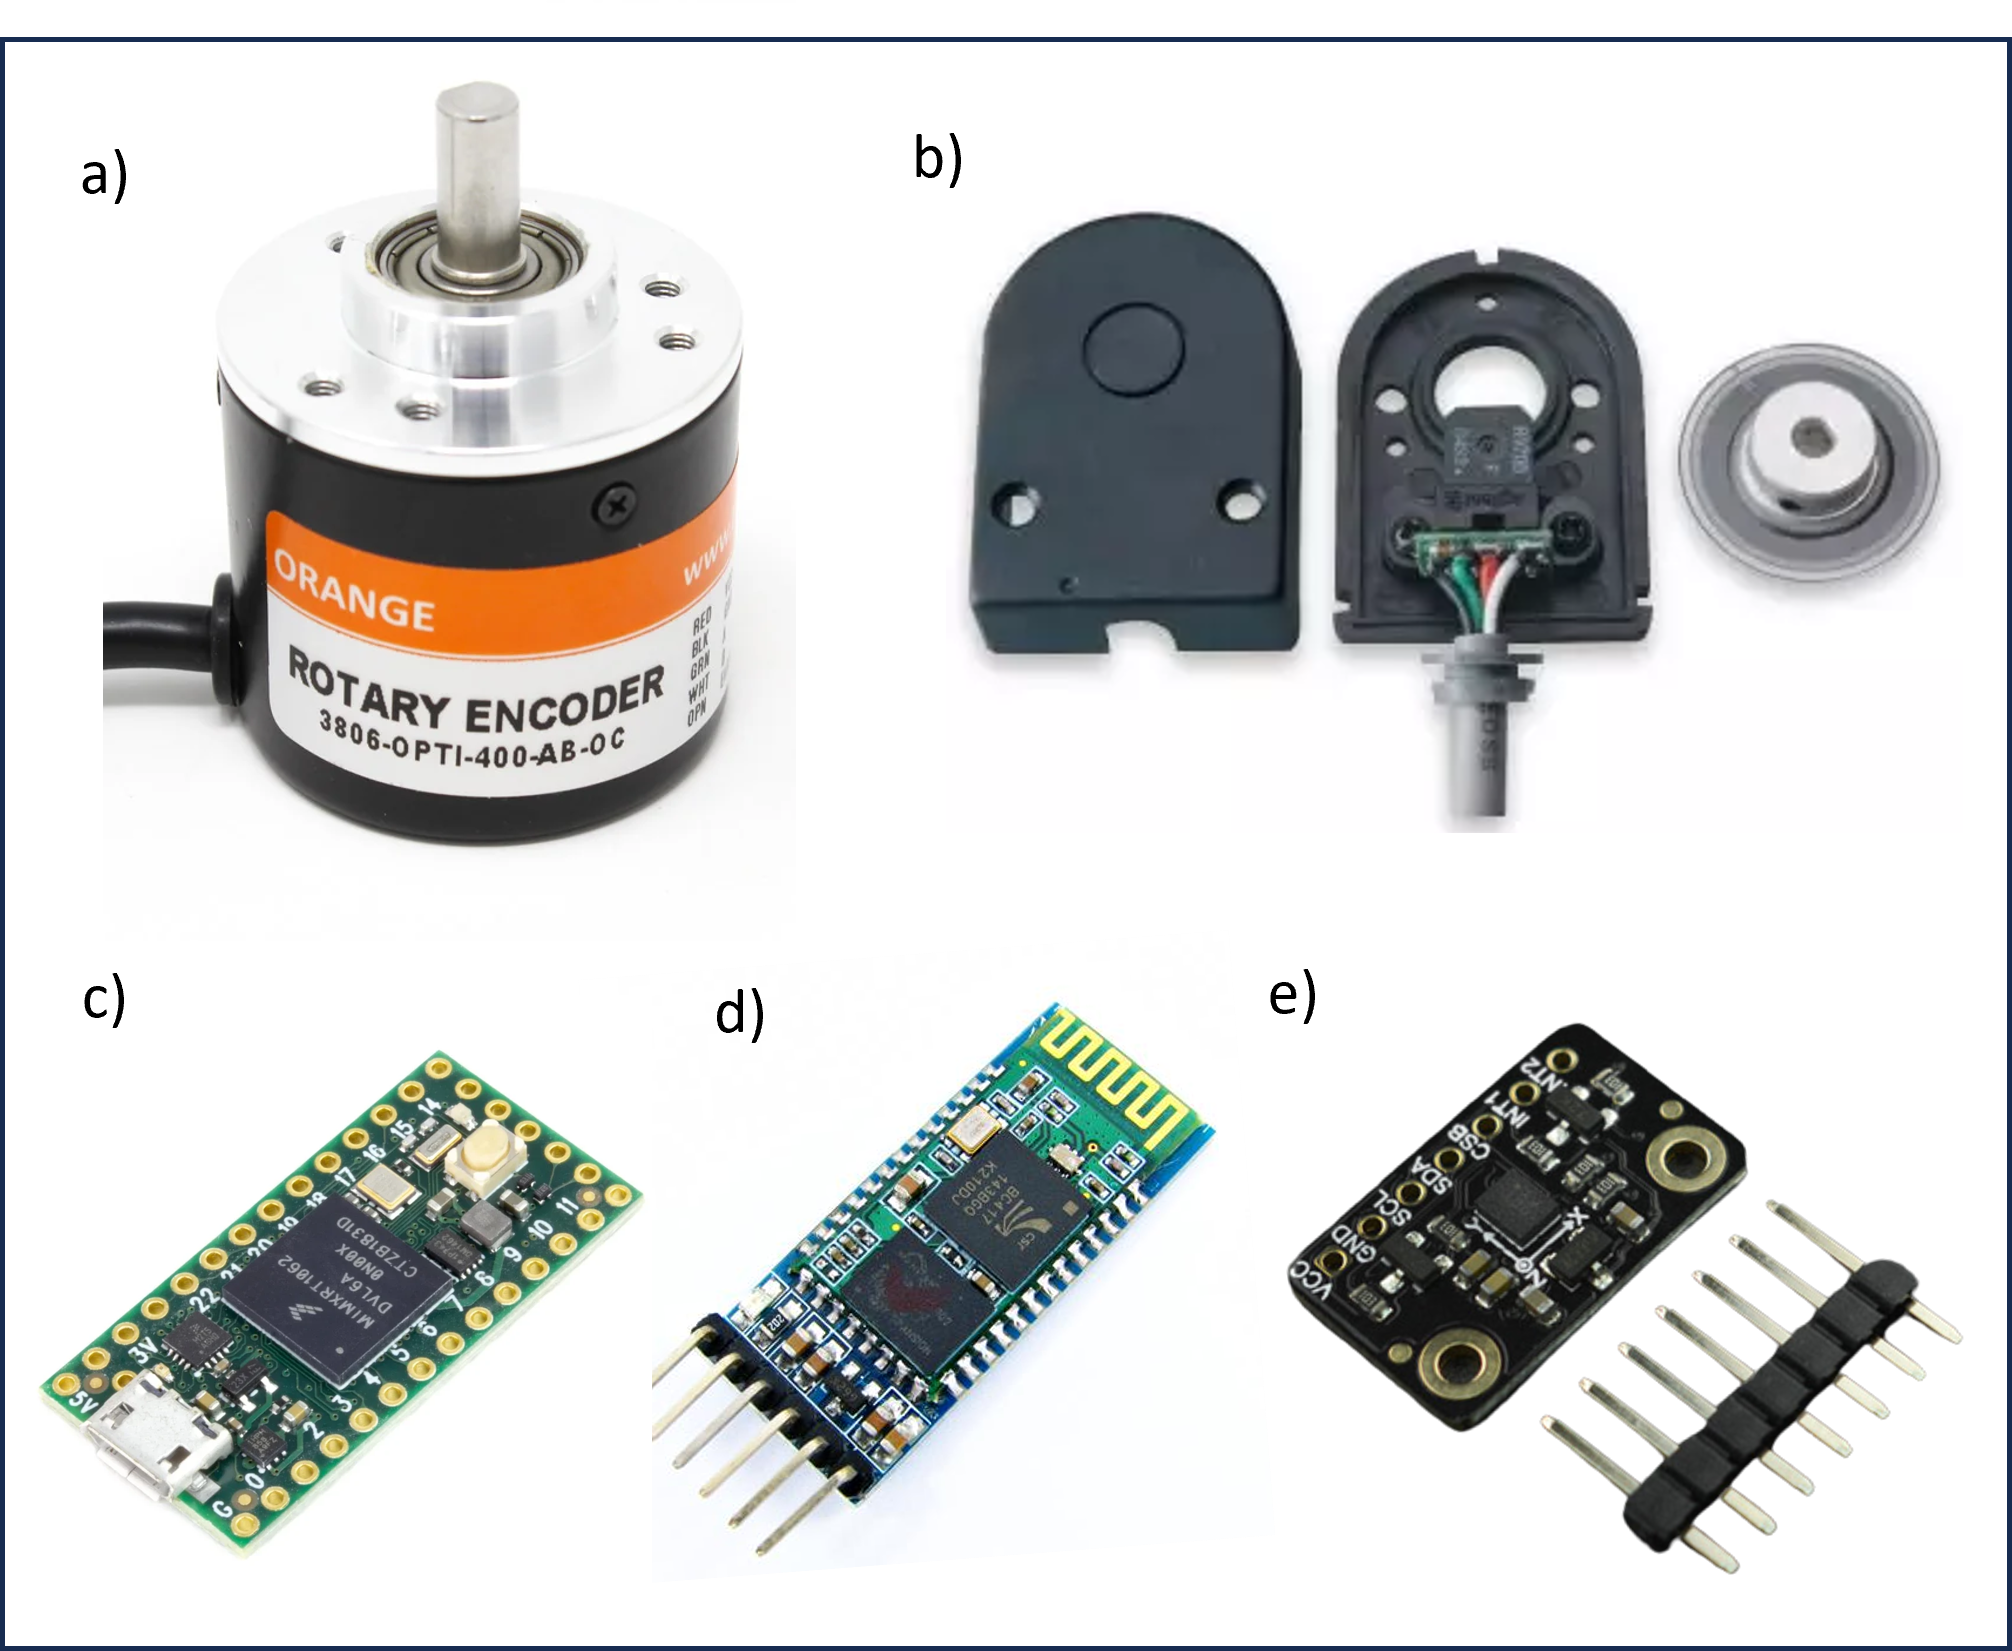
\includegraphics[width=\textwidth]{m_controller.png}
    \caption{ArmBo sensors}
    {a) Orange encoder, b) Hollow shaft encoder, c) Teensy 4.0
        d) HC-05 bluetooth module, e) DFRobotic BMX160 IMU
    }
    \label{fig:controller}
\end{figure}


\begin{figure}[hbt!]
    \centering
    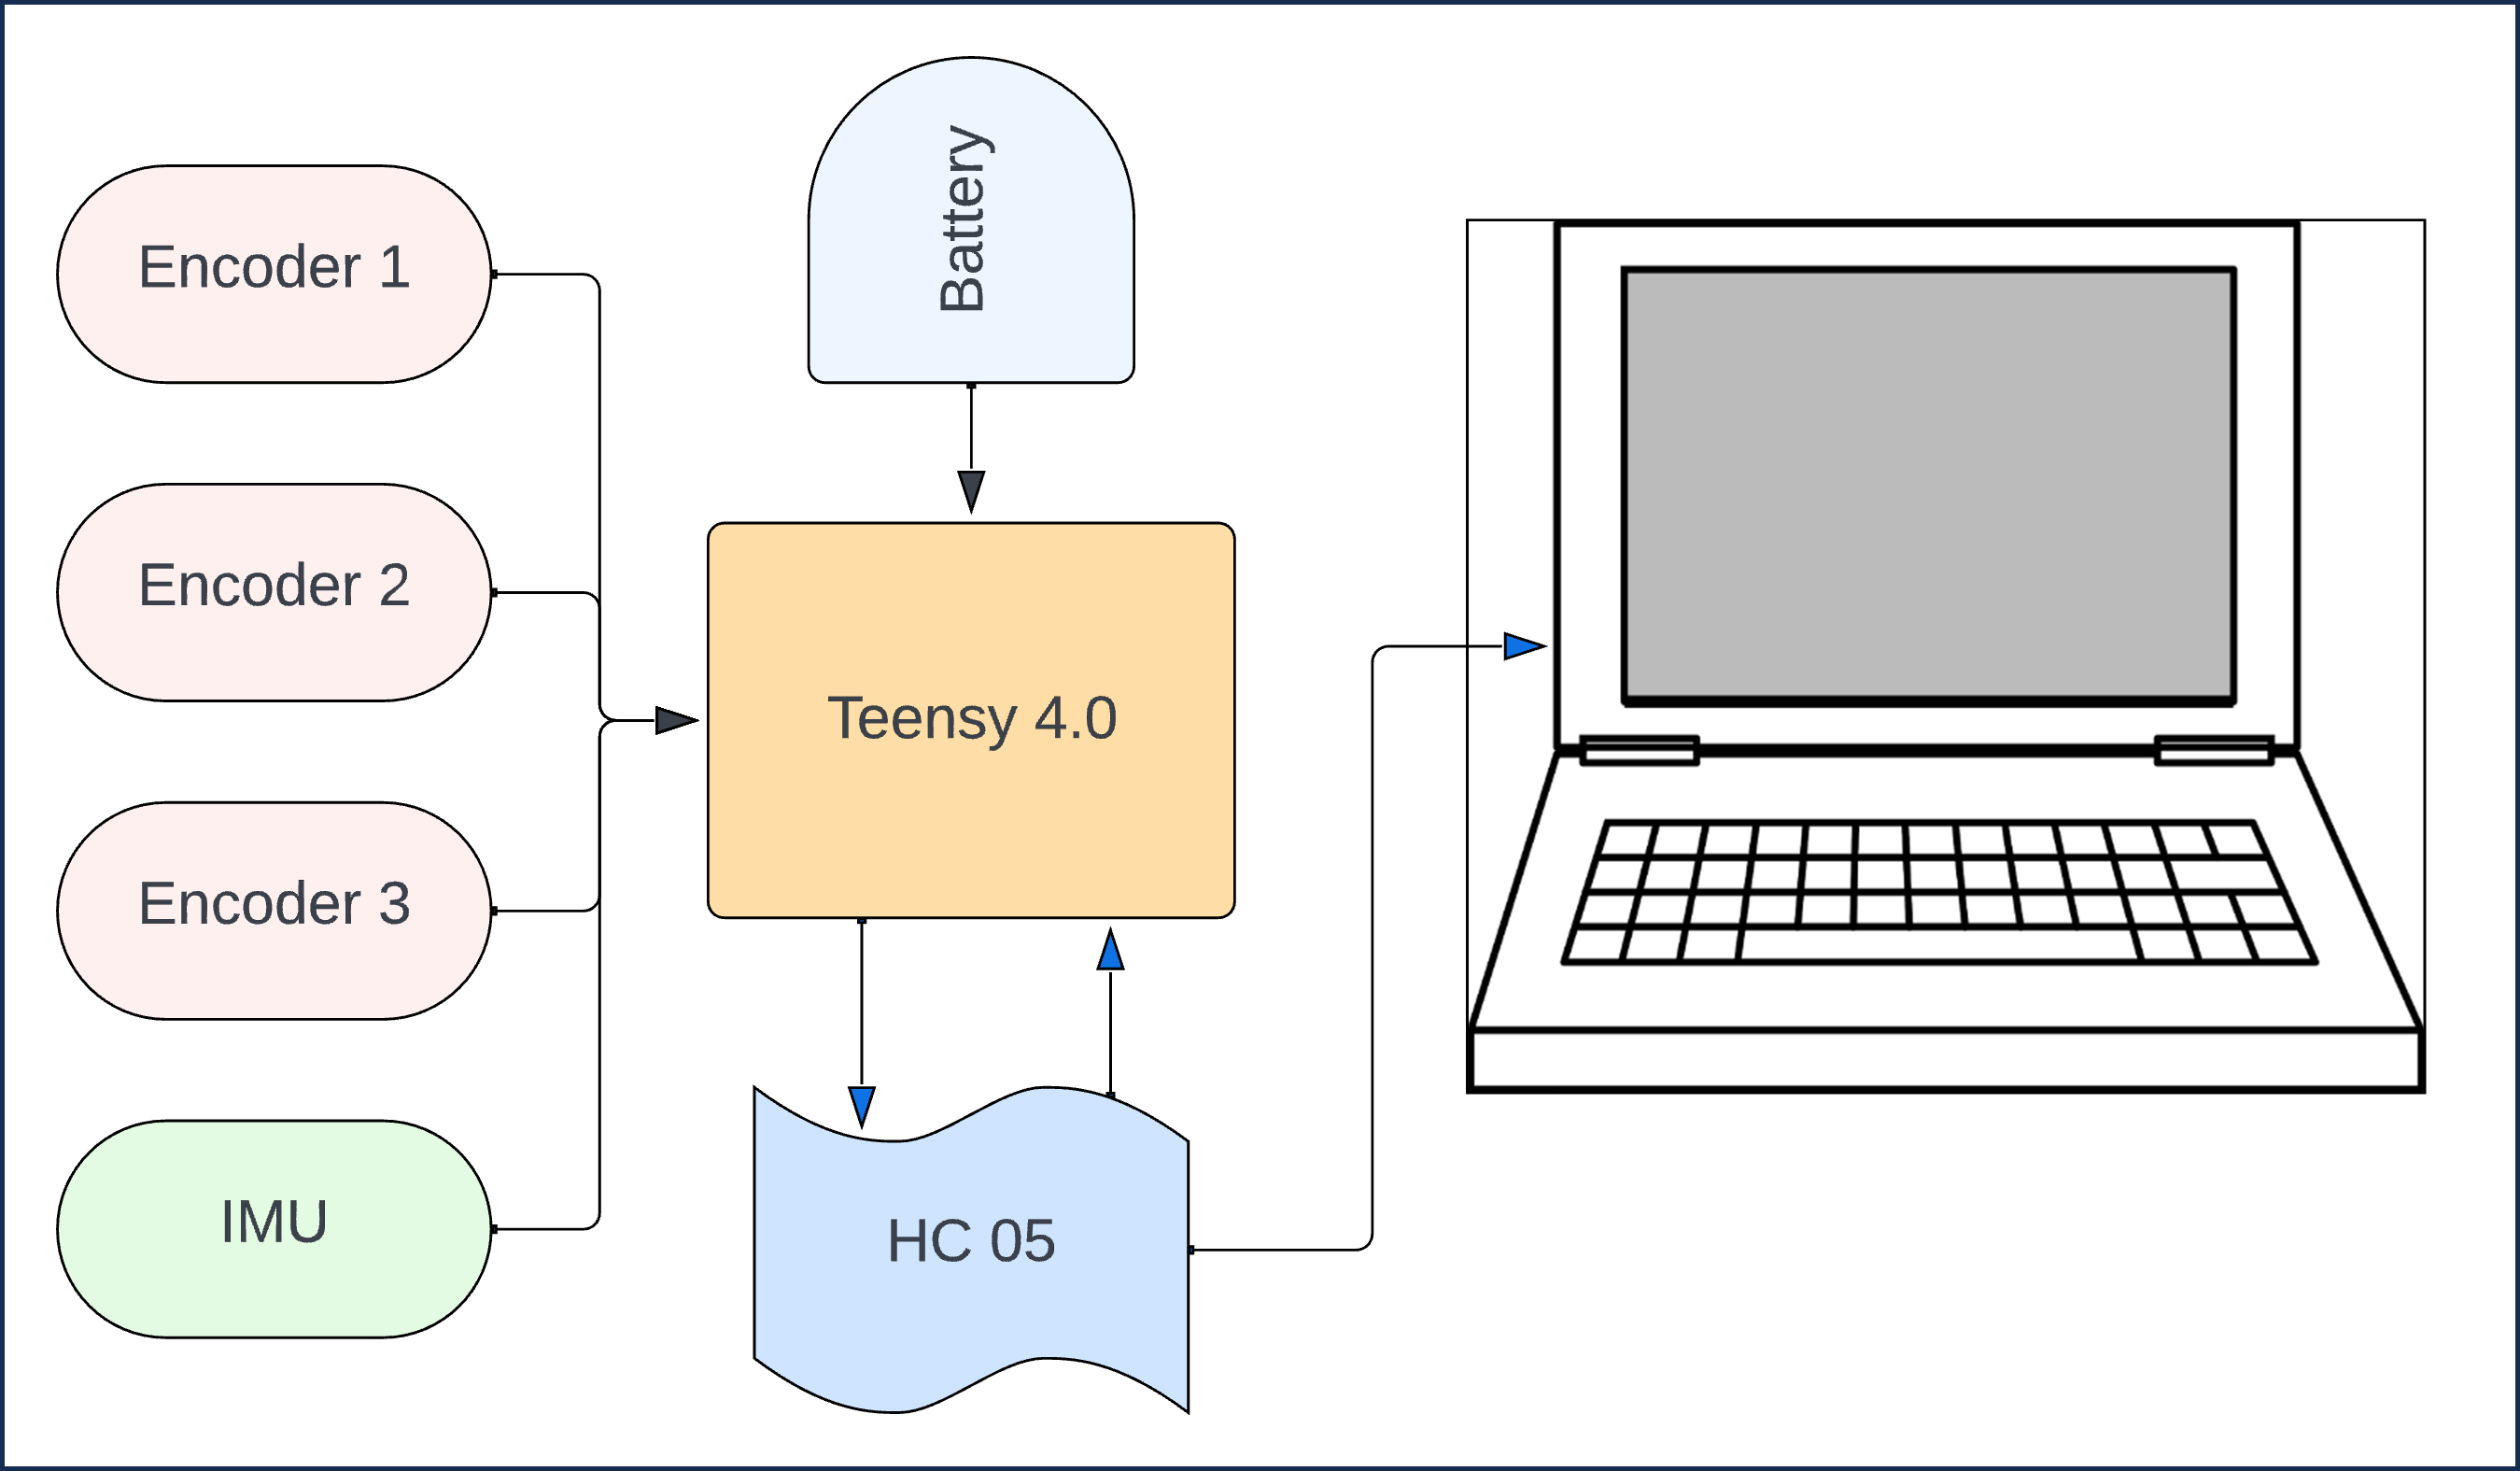
\includegraphics[width=\textwidth]{m_pcb_skematic.png}
    \caption{PCB skematic}
    \label{fig:pcb}
\end{figure}


\begin{figure}[hbt!]
    \centering
    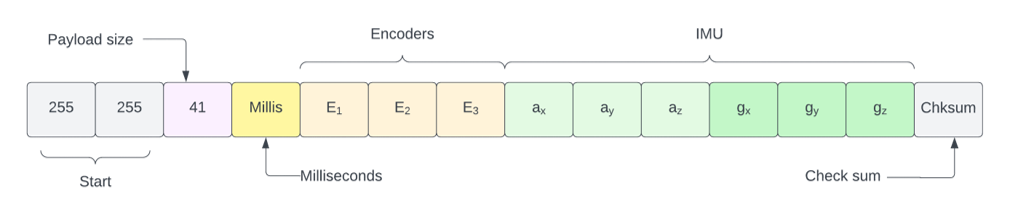
\includegraphics[width=\textwidth]{m_jedi.png}
    \caption{Communication protocol}
    {Total of 41 bytes are transmitted from the controller to the PC}
    \label{fig:jedi}
\end{figure}

\newpage
\section{Sensor validation}
\subsection{Encoder validation}

To ensure the accuracy of the optical encoders, the following experiment was conducted.
the encoder are mounted on a pro-circle as shown in \ref{fig:encoder_val}, and 20 rotations were made, to see any visual offset
is done by the encoder. The orange encoder performed better compared to hollow shaft encoder as shown in Fig \ref{fig:omniwheel} b,
Thus, we equiped the skateboard with Orange encoders.

\begin{figure}[hbt!]
    \centering
    \fbox{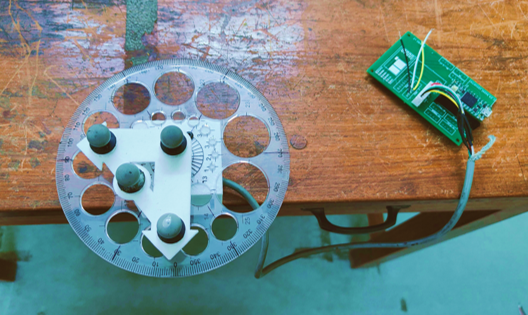
\includegraphics[width=0.8\textwidth]{m_encoder_val.png}}
    \caption{Encoder validation procedure}
    {Optical encoder are mounted on a pro-circle}
    \label{fig:encoder_val}
\end{figure}

\subsection{IMU validation}

Bosch IMU from DFRobotic is used for estimating the current orientation of the skateboard
in the real-world frame. The IMU is mounted on the skateboard as shown in Fig \ref{fig:imu_skematic} a.
The IMU is validated by rotating the skateboard in the real-world frame
and comparing the IMU estimated orientation with the ground truth orientation. The ground truth orientation
is obtained by using a motion capture system. The IMU validation experiment is shown in Fig \ref{fig:imu_val} b.
The IMU estimated orientation is compared with the ground truth orientation in Fig \ref{fig:imu_val} c. \\

\begin{figure}[h!]
    \centering
    \fbox{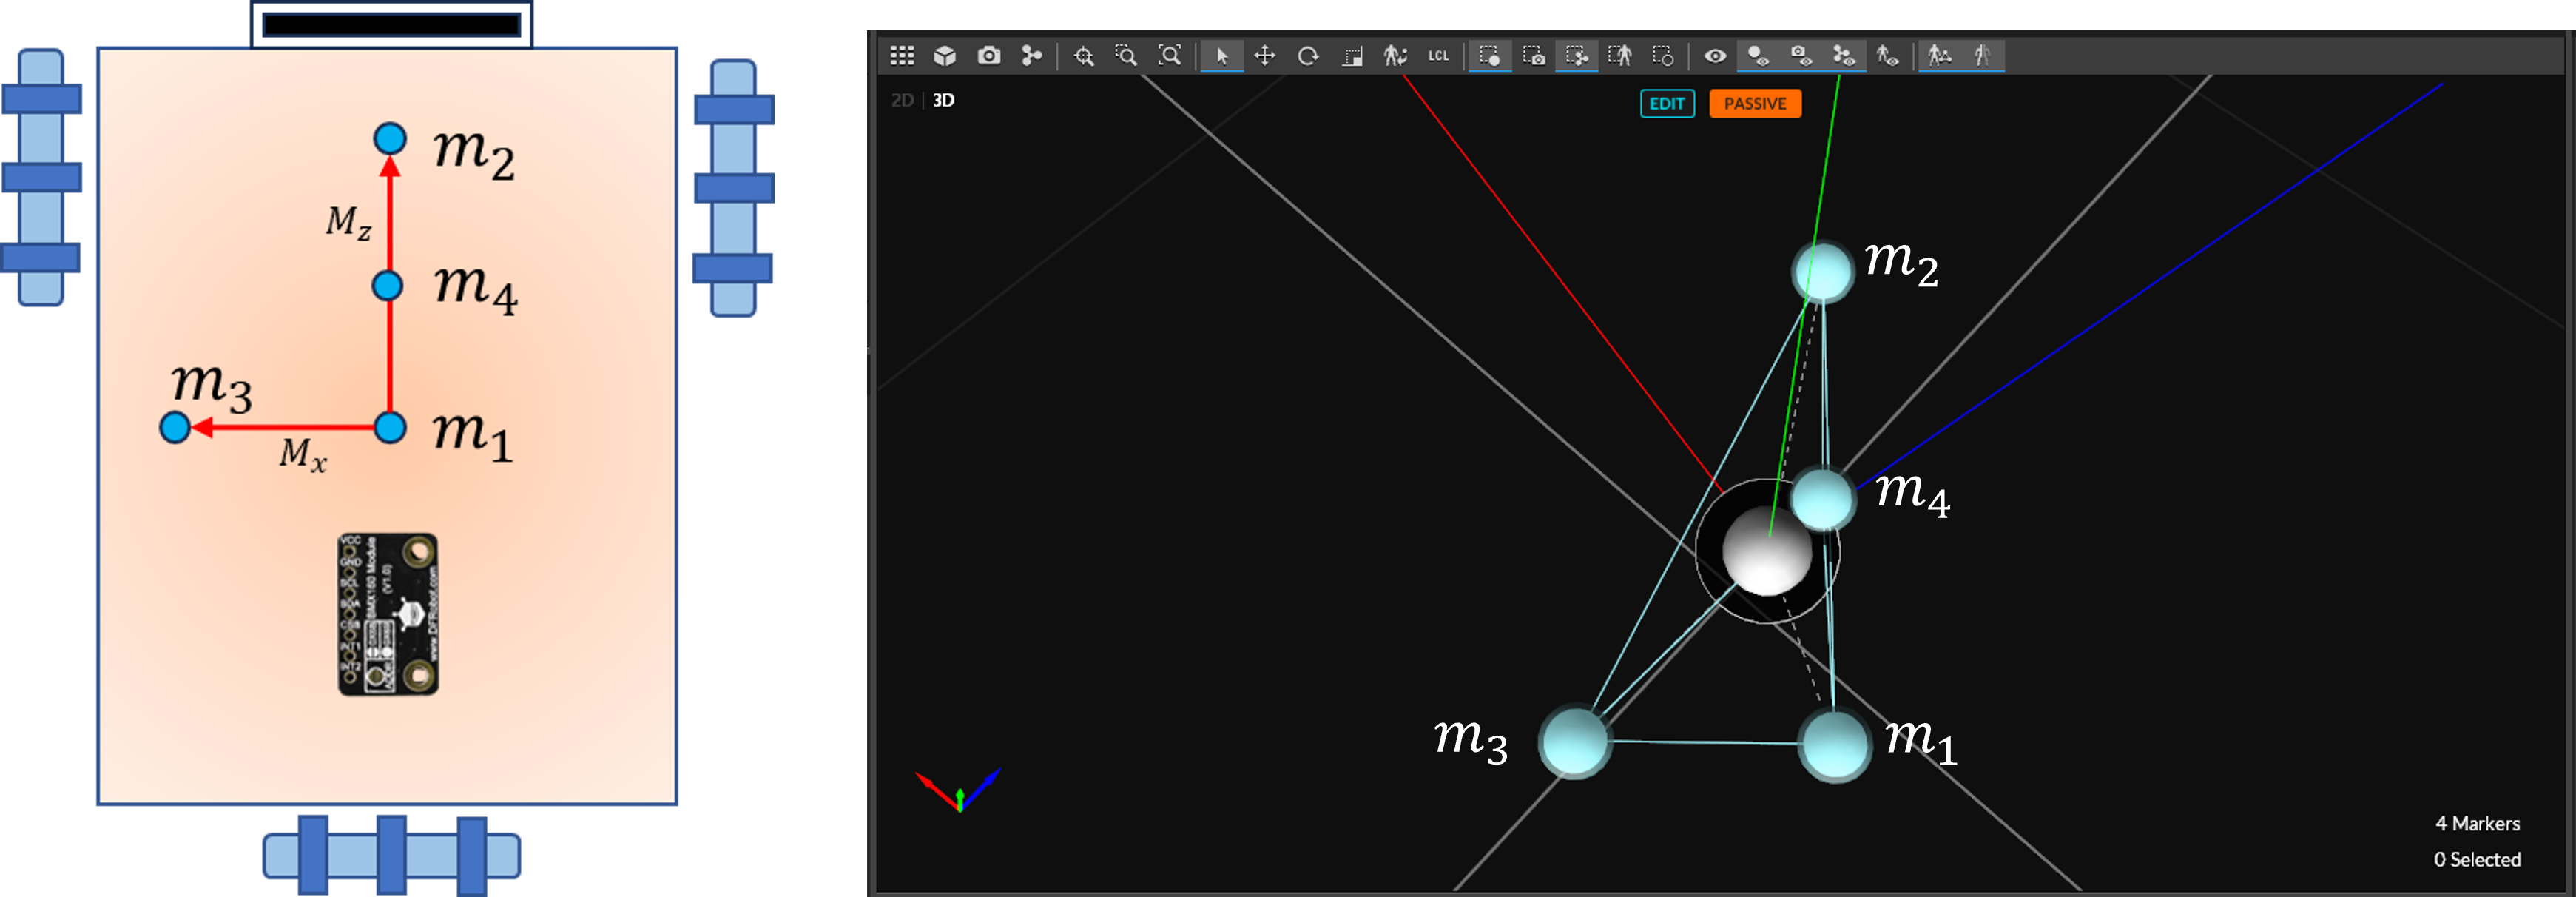
\includegraphics[width=\textwidth]{m_imu_skematic.png}}
    \caption{IMU Validation procedure}
    {a) Shows motion capture marker placement, IMU is fixed inside the skateboard, b) shows the ridig body representtion of Motion capture markers, in the OptiTrack
        motive software}
    \label{fig:imu_skematic}
\end{figure}

To determine the angle from the reflective markers, we used gram-schmidt process to find the rotation matrix
from the three markers $\begin{bmatrix}
        m_1 & m_2 & m_3
    \end{bmatrix}$, at each instant. This will result in a orthonormal reference frame for each instant. \\

The reference frame at time $t = 0$ is taken as the global frame, the global frame in inversed and multiplied with
the reference frame at time $t$, to get the rotation matrix at each instant.
The rotation matrix is then converted to euler angles, which is then compared with the IMU\\

We observed a maximum error of 5 degrees in the IMU estimated orientation, for 10 minute of recording, as shown
in Fig \ref{fig:imu_val}. We also observed that the IMU estimated orientation drifts over time,
which is a common issue with IMUs.


\begin{figure}[hbt!]
    \centering
    \fbox{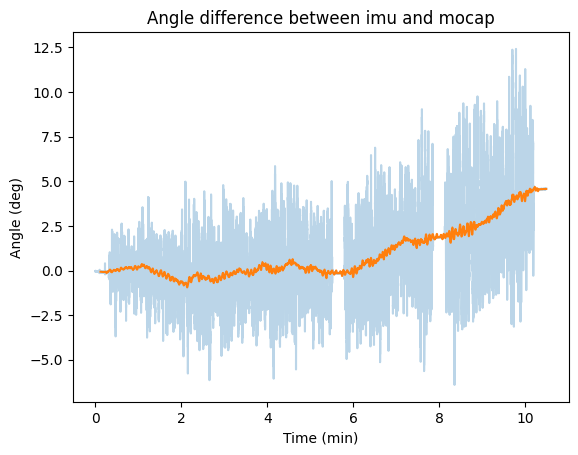
\includegraphics[width=0.9\textwidth]{m_imu_val.png}}
    \caption{IMU drift over time}
    {Error plot of IMU estimated orientation vs motion capture}
    \label{fig:imu_val}
\end{figure}



\newpage
\section{Investigation of encoder based approach}
\subsection{Deriving the kinematic model of ArmBo}

The position and orientation of ArmBo can potentially be determined by
developing its kinematic model. This generalized kinematic expression
is derived from the book “Modern Robotics Mechanics Planning and Control”
authored by Kevin M Lynch and Frank C Park.

An omnidirectional wheel has two components of velocity, one is the driving velocity
and the other is sliding velocity. The driving velocity is the velocity of the wheel
in the direction of the wheel axis. The sliding velocity is the velocity of the wheel
in the direction perpendicular to the wheel axis.

Minimum of three omnidirectional wheels are required, to determine its three-dimentional
chasis velocity $\dot{q} = (\dot{\phi}, \dot{x}, \dot{y}) $

\begin{figure}[h!]
    \centering
    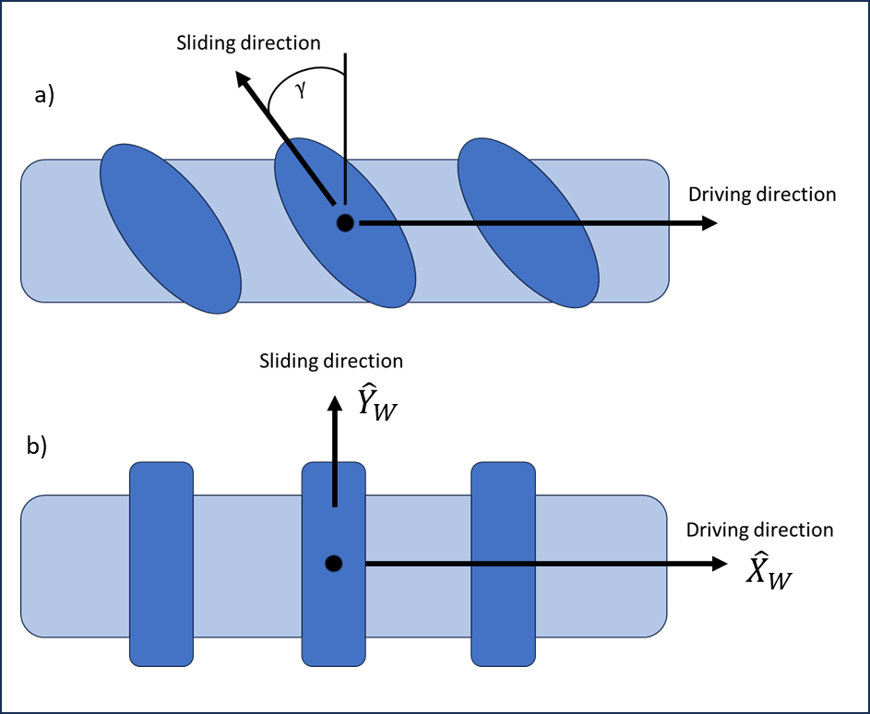
\includegraphics[width=0.8\textwidth]{m_wheel_kinematic.png}
    \caption{Omnidirectional wheel kinematic model}
    {a Mecanum wheel directional velocities, b:omnidirectional wheel directional velocities}
    \label{fig:wheel_kinematic}
\end{figure}


From a frame $\hat{X}_W - \hat{Y}_W$, the linear velocity of the center of the onmiwheel is
written as $v = (v_x, v_y)$.

\begin{equation}
    \begin{bmatrix}
        v_x \\ v_y
    \end{bmatrix}
    =
    v_{drive} \begin{bmatrix}
        1 \\ 0
    \end{bmatrix}
    +
    v_{slide} \begin{bmatrix}
        -\sin{\gamma} \\ \cos{\gamma}
    \end{bmatrix}
\end{equation}

Here, $\gamma$ is the angle at which the passive rollers are oriented,
which allows free sliding. \\

Thus, generalized expression for single omnidirectional wheel is
\newline

$u_i  = h_i (\phi) \dot{q} =  $


\begin{equation}
    h_1(0) \mathcal{V}_b = \frac{1}{r_i} \left[\begin{array}{cc}
            1 & \tan\gamma_i \\
        \end{array}\right]
    \left[\begin{array}{cc}
            \cos \beta_i  & \sin \beta_i \\
            -\sin \beta_i & \cos \beta_i \\
        \end{array}\right]
    \begin{bmatrix}
        -y_i & 1 & 0 \\
        x_i  & 0 & 1 \\
    \end{bmatrix} \mathcal{V}_b
\end{equation}

As shown in Fig \ref{fig:kinematic_shematic} for the first
wheel $w_1$, $\gamma_1 = 0, \beta_1 = \frac{\pi}{2}$ so, the expression becomes

\begin{figure}[hbt!]
    \centering
    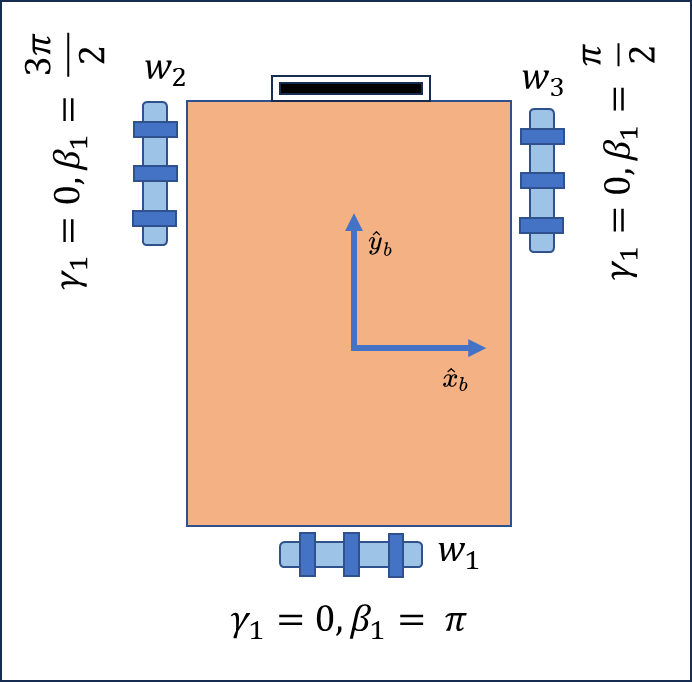
\includegraphics[width=0.8\textwidth]{m_kinematic_shematic.png}
    \caption{Skateboard local frame of reference}
    {asdf}
    \label{fig:kinematic_shematic}
\end{figure}


\begin{equation}
    = \frac{1}{r_1}
    \begin{bmatrix}
        1 & 0 \\
    \end{bmatrix}
    \begin{bmatrix}
        \cos \frac{\pi}{2}  & \sin \frac{\pi}{2} \\
        -\sin \frac{\pi}{2} & \cos \frac{\pi}{2} \\
    \end{bmatrix}
    \begin{bmatrix}
        -y_1 & 1 & 0 \\
        x_1  & 0 & 1 \\
    \end{bmatrix}
    \mathcal{V}_b
\end{equation}


\begin{equation}
    = \frac{1}{r_1} \left[\begin{array}{cc}
            1 & 0 \\
        \end{array}\right]
    \begin{bmatrix}
        0  & 1 \\
        -1 & 0 \\
    \end{bmatrix}
    \begin{bmatrix}
        -y_1 & 1 & 0 \\
        x_1  & 0 & 1 \\
    \end{bmatrix}
    \mathcal{V}_b
\end{equation}

\begin{equation}
    = \frac{1}{r_1} \left[\begin{array}{cc}
            1 & 0 \\
        \end{array}\right]
    \begin{bmatrix}
        -x_1 & 0 & 1 \\
        -y_1 & 1 & 0 \\
    \end{bmatrix}
    \mathcal{V}_b
\end{equation}

\begin{equation}
    =
    \frac{1}{r_i}
    \begin{bmatrix}
        -x_1 & 0 & 1 \\
    \end{bmatrix}
    \mathcal{V}_b
\end{equation}

\begin{equation}
    r_i = r_1 = r_2 = r_3 = r
\end{equation}

Thus, the expression for the first wheel is

\begin{equation}
    h_2(0) \mathcal{V}_b = \frac{1}{r}
    \begin{bmatrix}
        x_2 & 0 & 1 \\
    \end{bmatrix}
    \mathcal{V}_b
\end{equation}

% for 2nd wheel
% bold text here

Similarly for the second wheel, where $\gamma_2 = 0, \beta_2 = \frac{3\pi}{2}$

\begin{equation}
    h_3(0) \mathcal{V}_b = \frac{1}{r}
    \begin{bmatrix}
        -x_3 & 0 & -1 \\
    \end{bmatrix}
    \mathcal{V}_b
\end{equation}


% for 3rd wheel
% bold text here

Similarly for the third wheel

\begin{equation}
    h_1(0) \mathcal{V}_b = \frac{1}{r}
    \begin{bmatrix}
        y_1 & -1 & 0 \\
    \end{bmatrix}
    \mathcal{V}_b
\end{equation}


We know that

\begin{equation}
    y = y_1,  x_2 = -x_3
\end{equation}

The final expression for the three wheel omnidirectional robot is

\begin{equation}
    H(0)\mathcal{V}_b = \frac{1}{r}
    \begin{bmatrix}
        y  & -1 & 0 \\
        -x & 0  & 1 \\
        x  & 0  & 1 \\
    \end{bmatrix}
    \begin{bmatrix}
        \omega_{bz}   \\
        \upsilon_{bx} \\
        \upsilon_{by} \\
    \end{bmatrix}
\end{equation}

To find
$
    \begin{bmatrix}
        \omega_{bz}   \\
        \upsilon_{bx} \\
        \upsilon_{by} \\
    \end{bmatrix}
$\\

% insert symbol
Lets insert the symbol for the above expression
\begin{align}
    \mathcal{A}  =
    \begin{bmatrix}
        y  & -1 & 0 \\
        -x & 0  & 1 \\
        x  & 0  & 1 \\
    \end{bmatrix}
\end{align}


To find
$
    \begin{bmatrix}
        \omega_{bz}   \\
        \upsilon_{bx} \\
        \upsilon_{by} \\
    \end{bmatrix}
$ = $r\mathcal{A}^{-1} u$

The directional velocity, and angular velocity are then converted to displacement and angular displacement
and compared against
the ground truth position and orientation.

\subsection{Accuracy of the Encoder based approach}
The accuracy of the encoder based approach is validated by comparing the
estimated position and orientation of ArmBo with the ground truth position and orientation.
The ground truth position and orientation is obtained by using a motion capture system.

The duration of the experiment is 10 minutes, and the sampling frequency of the sensors is  set to 100 Hz.
The results are shown in Fig \ref{fig:enc_val_coord}. The error between the estimated and ground truth position
are drifting over time. This can be due to various reasons, such as wheel slippage, or the skateboard
being lifted off the ground. This has also been discussed by variour authors, this is a common issue with
an odometry based system.


\begin{figure}[hbt!]
    \centering
    \fbox{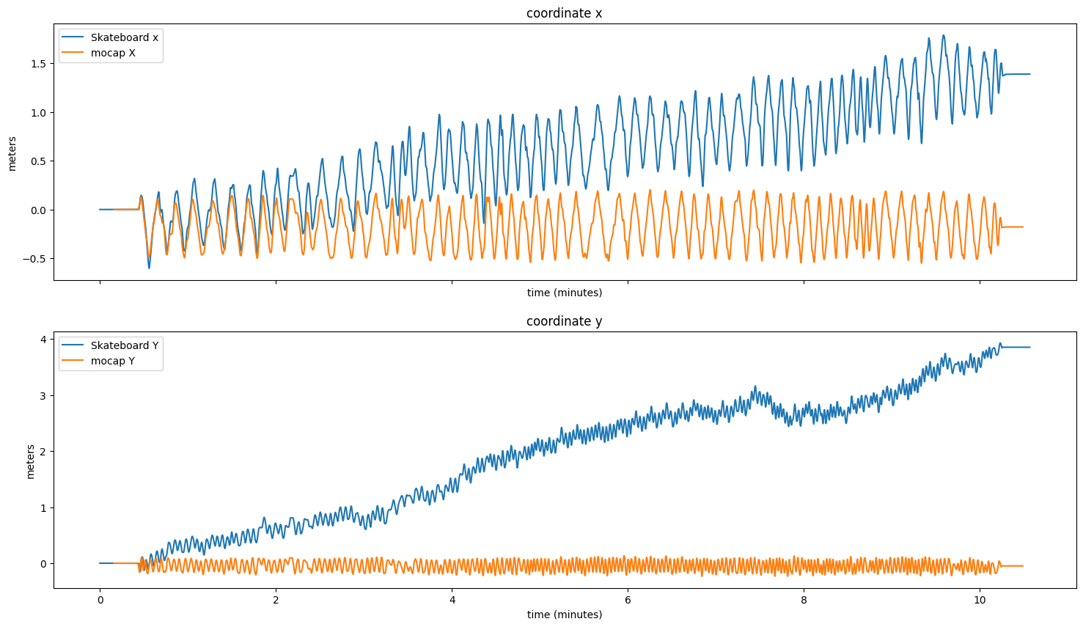
\includegraphics[width=\textwidth]{m_enc_coord.png}}
    \caption{Encoder based coordinate vs motion capture}
    {a) X coordinate, b) Y coordinate}
    \label{fig:enc_val_coord}
\end{figure}


\begin{figure}[h!]
    \centering
    \fbox{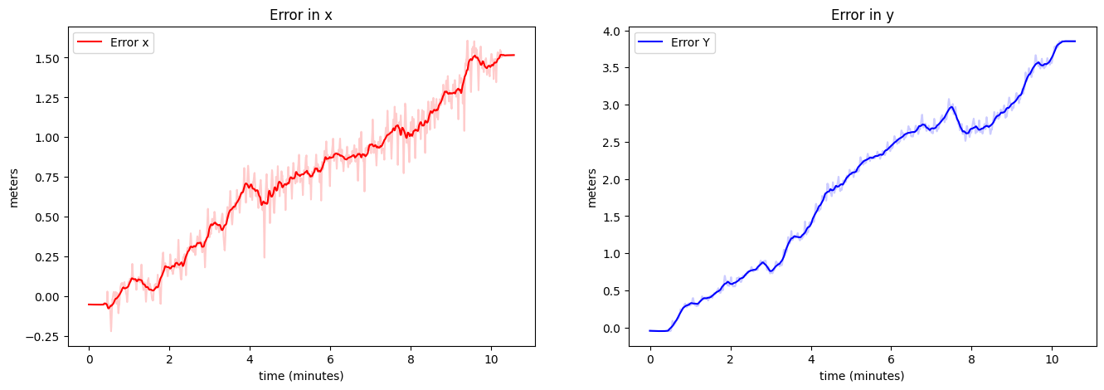
\includegraphics[width=\textwidth]{m_enc_coord_err.png}}
    \caption{Error plot of encoder based coordinate vs motion capture}
    {a) X coordinate, b) Y coordinate}
    \label{fig:enc_val_coord_err}
\end{figure}


\begin{figure}[h!]
    \centering
    \fbox{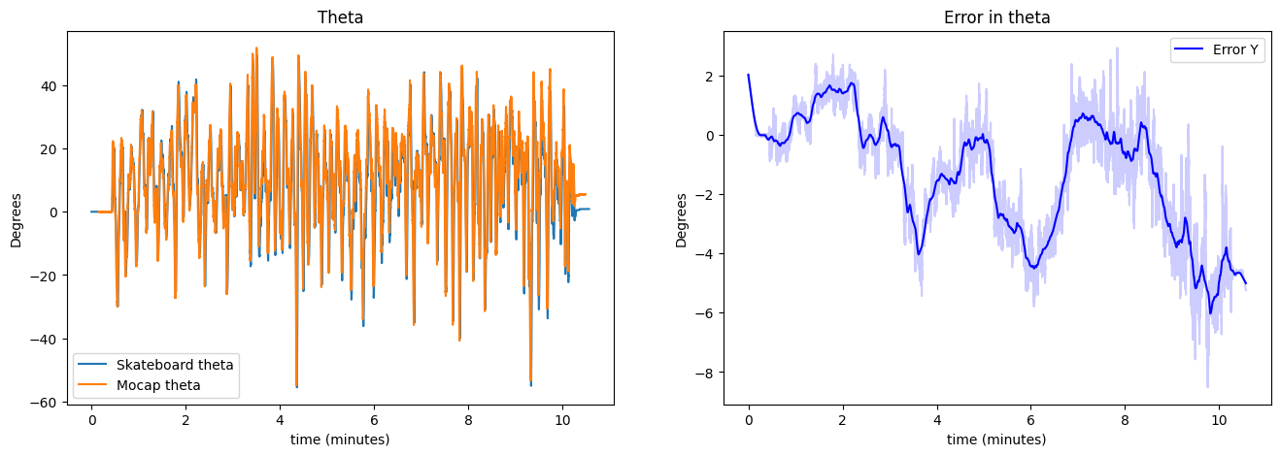
\includegraphics[width=\textwidth]{m_theta.png}}
    \caption{Validatoin of angle estimates from encoder}
    {a) ArmBo vs mocap angle, b) Error plot of ArmBo vs mocap angle}
    \label{fig:enc_theta}
\end{figure}

\section{Investigation of Camera based approach using ArUco marker}

\subsection{Calibration and reference frame of ArUco marker}

Calibration of ArUco marker is done through an ArUco board,
12 markers 5cm height and width with 1 cm spacing.
A video recording was done placing the ArUco board in different
orientations. And a random of 150 – 180 frames were used,
for best calibration pose accuracy result.
From that we drive camera intrinsic and extrinsic parameters are
calculated.


After calibration of the OptiTrack system, reference planes of both
ArUco and OptiTrack system are located using custom designed L-frame.

There are three ArUco markers (IDs = 0, 1, 2) placed orthogonally
in the custom designed L-frame as shown in FIG,
this will be referred to as ArUco L-Frame (ALF) in the
following sections. The ALF has three reflective markers
placed orthogonally for the OptiTrack mocap system, this is
referred to as Mocap L-frame. These two L-frames have a translational
offset of this much in X, Y, Z axis respectively.

The mocap global reference frame is located through
the OptiTrack proprietary Motive v2.2 software,
the ArUco marker are located and
orthogonalized using Gram-smith orthogonalization procedure.


\begin{figure}[h!]
    \centering
    \fbox{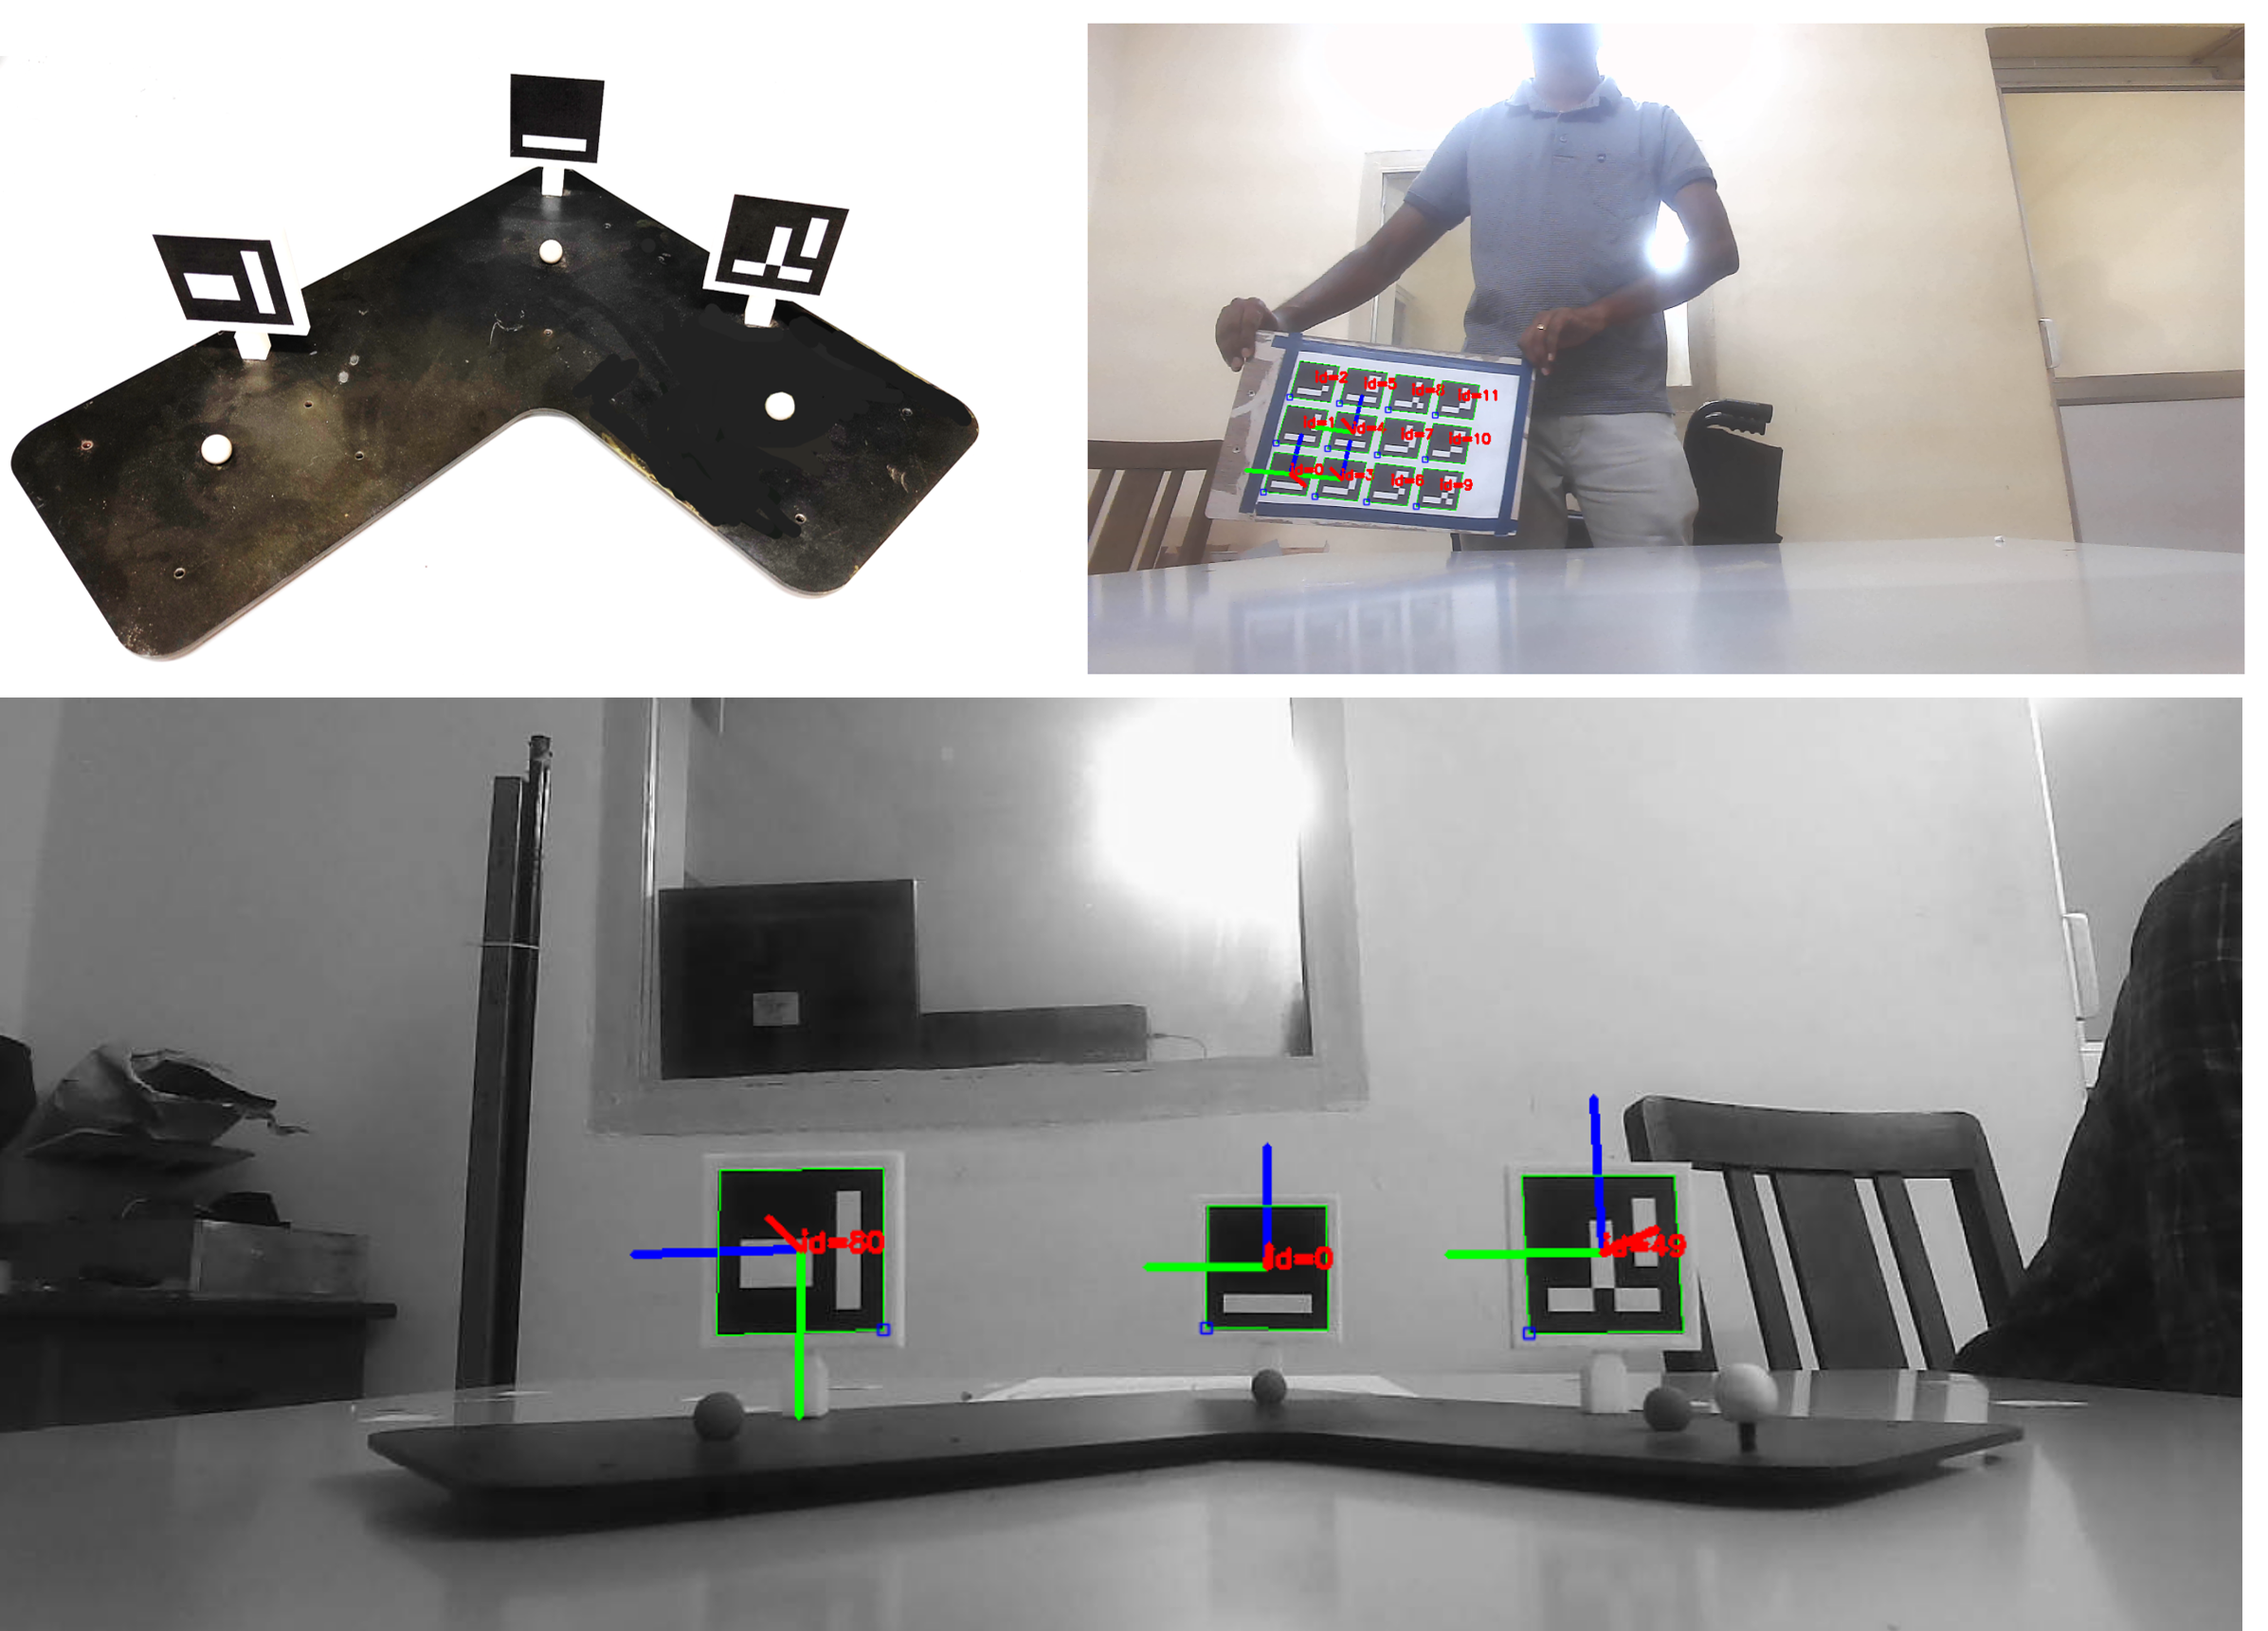
\includegraphics[width=\textwidth]{m_lframe.png}}
    \caption{Calibration procedure}
    {a) ArUco marker and motion capture global reference frame (L frame),
        b) ArUco marker calibration board, c) detection of L frame in the camera frame}
    \label{fig:lframe}
\end{figure}


\subsection{ArUco marker detection}
The ArUco marker detection is done using OpenCV library. The marker is placed
in front of the skateboard, and the camera is mounted on the table as shown in Fig \ref{fig:ar_mc} a.

The skateboard
is moved at different speeds and a fixed direction, Fig \ref{fig:ar_vel} b shows, the detection
of ArUco marker at different speeds. The ArUco marker is detected at a maximum speed of 0.3 m/s,
above which the marker is not detected. This is due to the motion blur, caused due to comparatively
high speed of the skateboard. The overall missing percentage of the ArUco marker is 27.5\%.


\begin{figure}
    \centering
    \fbox{\includegraphics[width=0.9\textwidth]{m_ar_mc.png}}
    \caption{ArUco marker validation}
    {a) ArUco marker facing the camera placed on the table,
        b) reflective markers placed on each corners of the ArUco marker,
        c) ridig body representation of the ArmBo in the OptiTrack motive software}
    \label{fig:ar_mc}
\end{figure}


\begin{figure}[hbt!]
    \centering
    \fbox{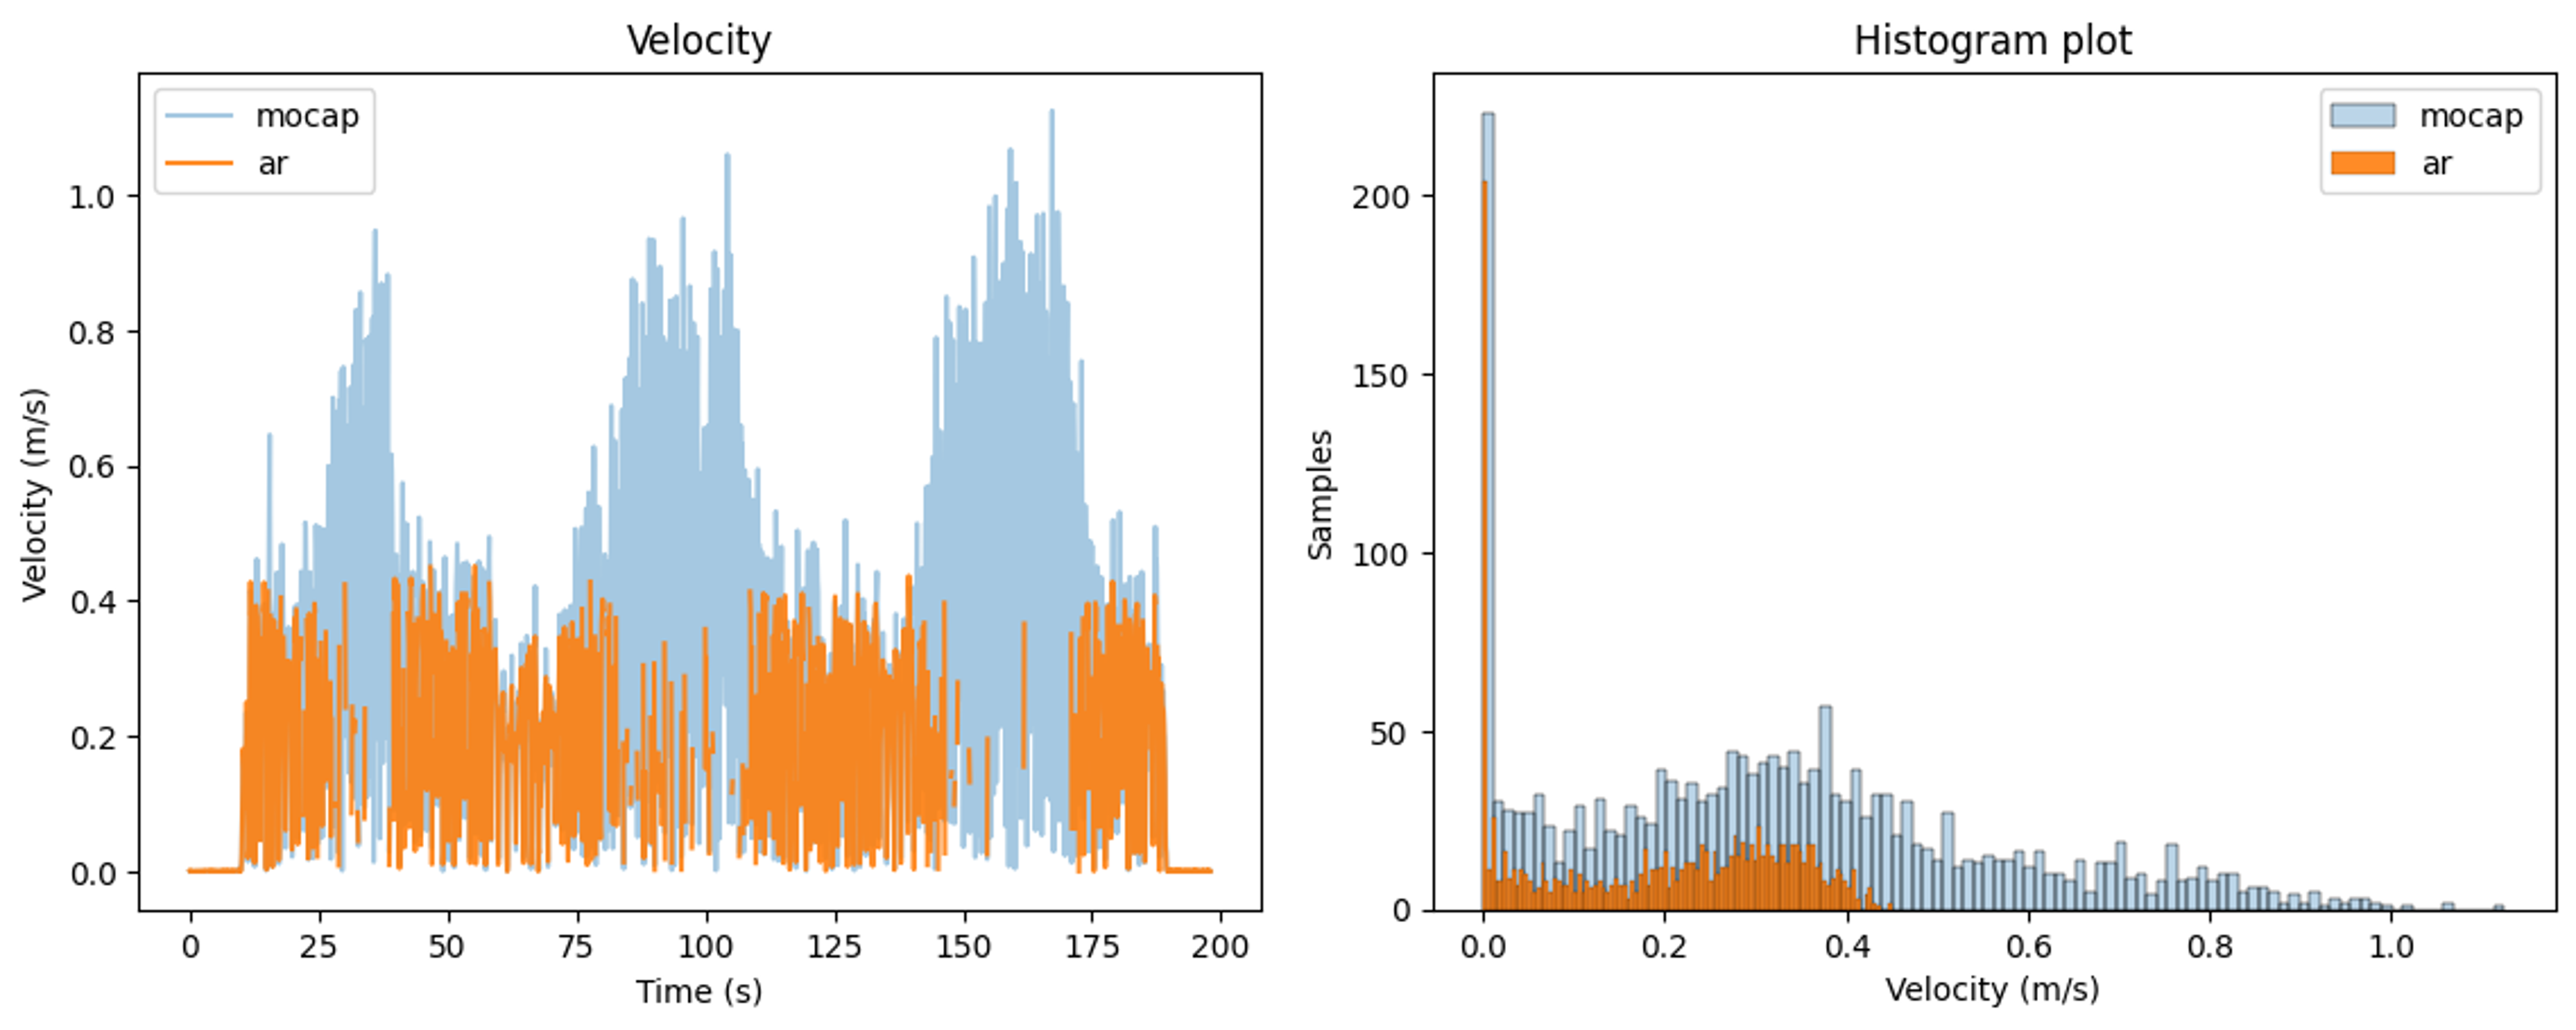
\includegraphics[width=\textwidth]{m_ar_vel.png}}
    \caption{ArUco marker detection based on speed}
    {a) ArUco marker velocity vs time,
        b) Histogram plot of ArUco marker detection based on velocity}
    \label{fig:ar_vel}
\end{figure}



\subsection{ArUco marker pose estimation}

To estimate the pose, we provide Camera Matrix and Distortion Coefficients,
to the solvePnP function in OpenCV. The solvePnP function takes in the 3D points
of the ArUco marker and the 2D points of the ArUco marker in the image frame,
and returns the rotation and translation vector of the ArUco marker in the camera frame.

The rotation and translation vector of the ArUco marker in the camera frame is then
converted to the rotation and translation matrix of the ArUco marker in the global L frame
as shown in Fig \ref{fig:lframe}.

The transformed coordinates of the ArUco marker in the global L frame is then compared with
the from the Motion capture sytem.

\begin{figure}[hbt!]
    \centering
    \fbox{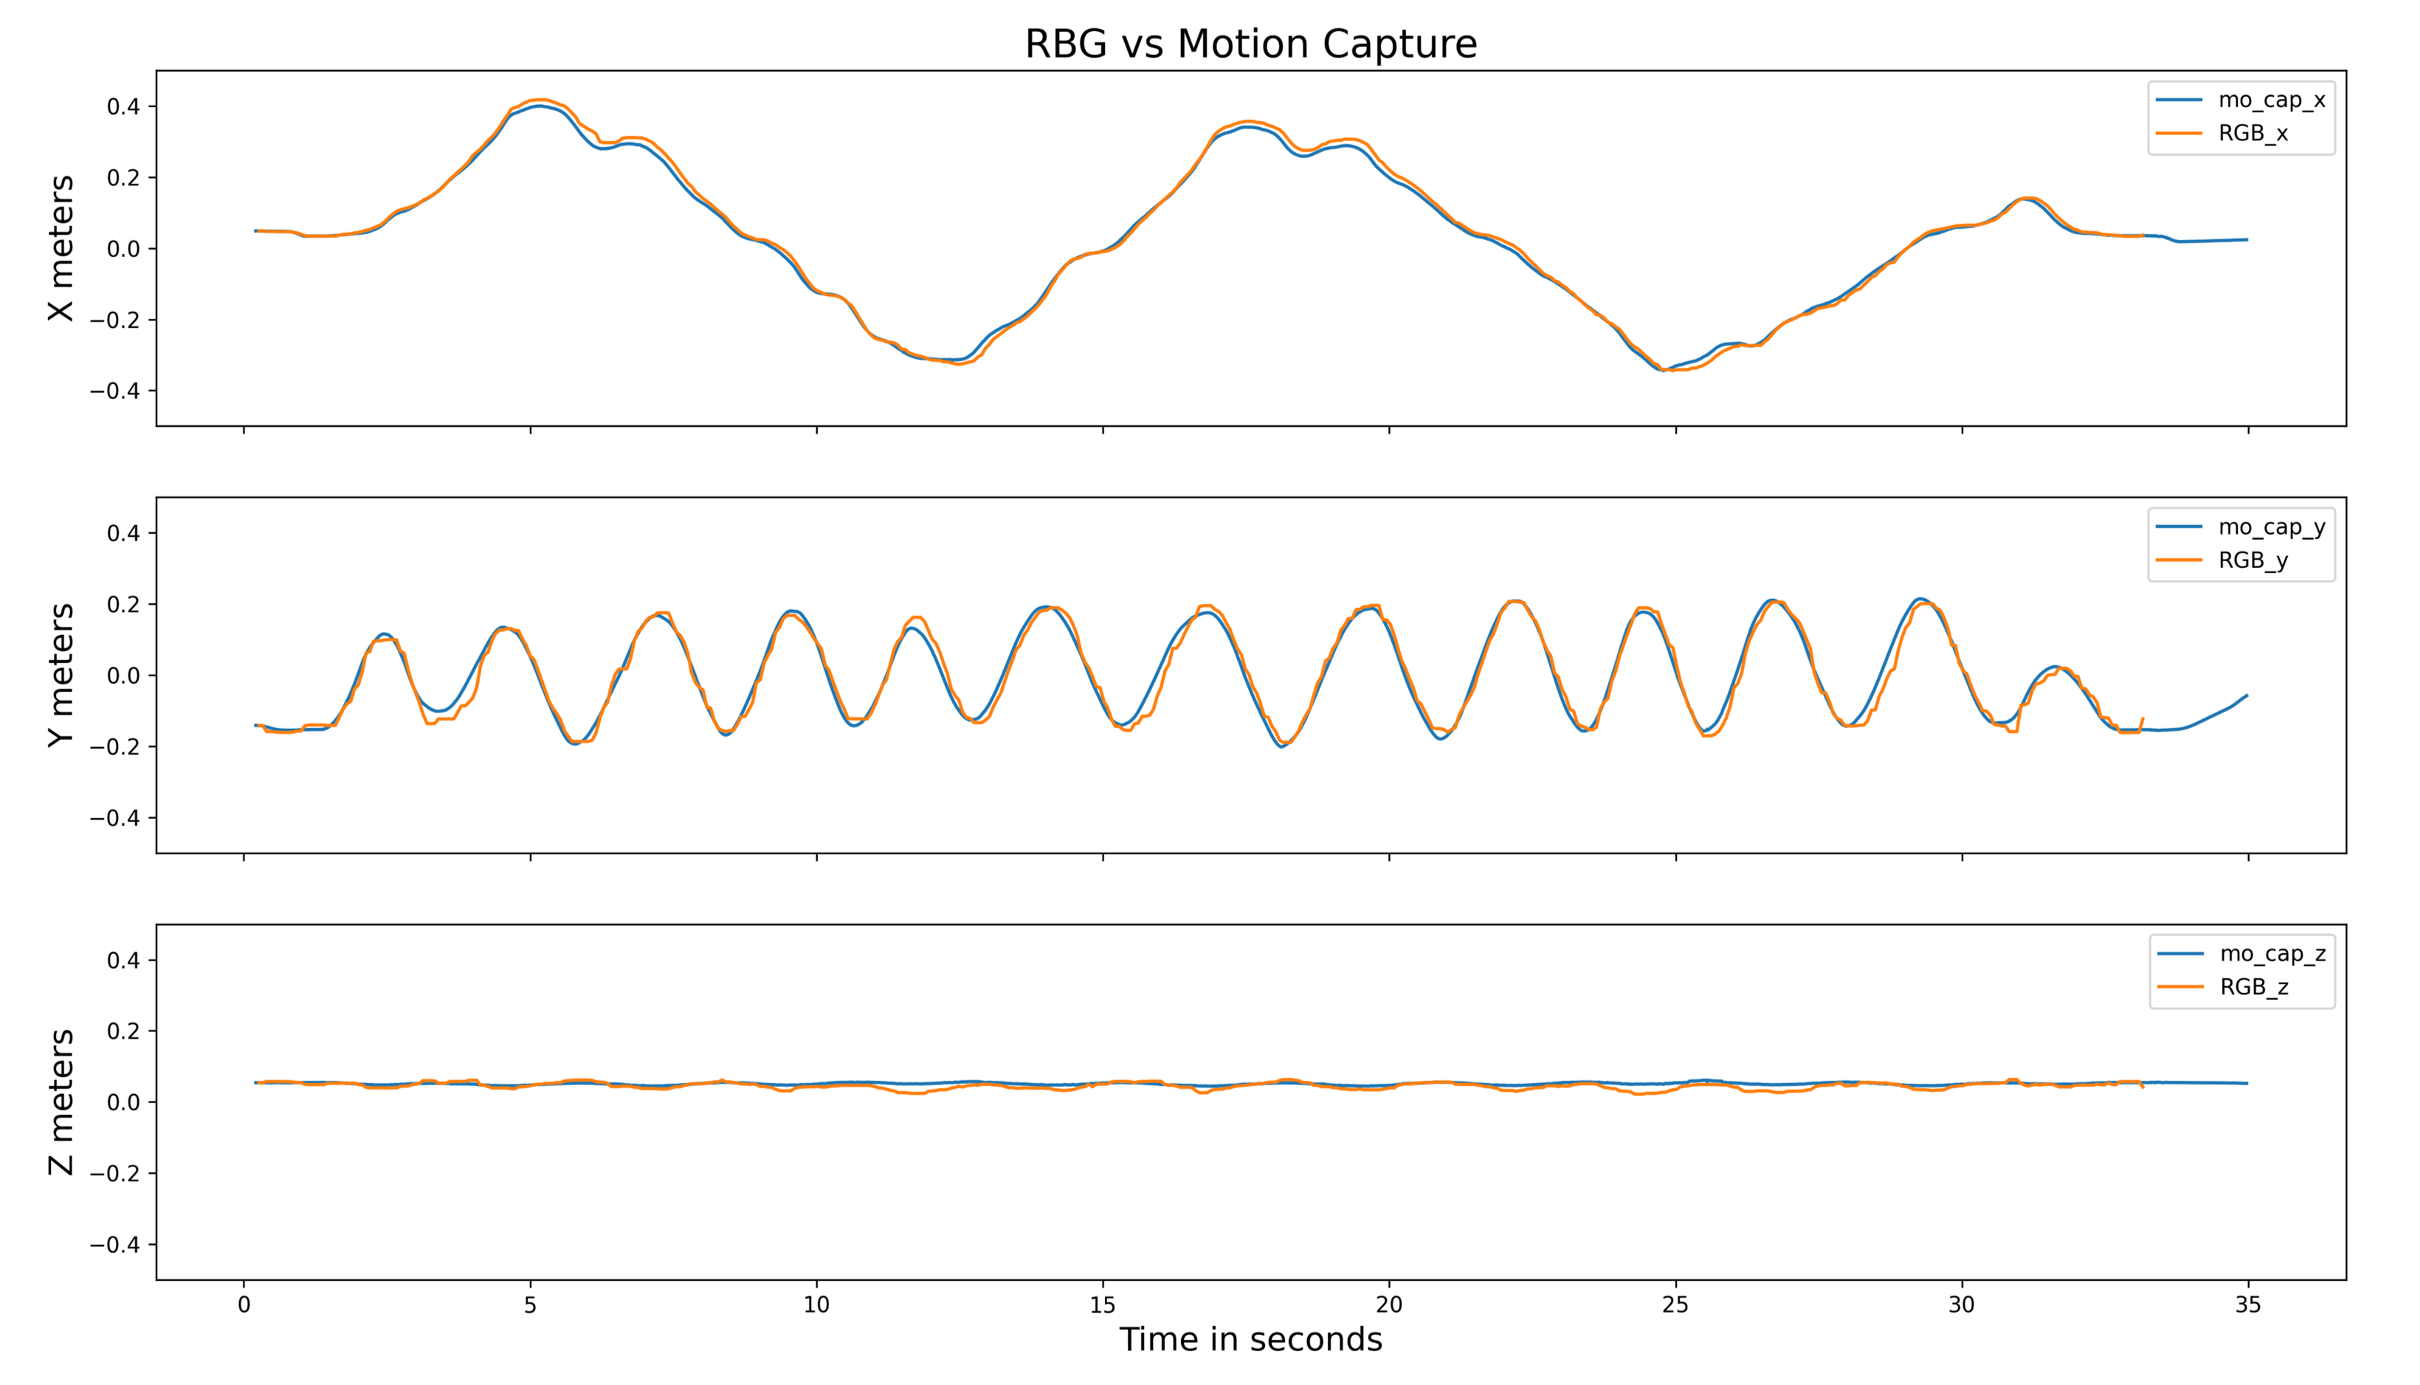
\includegraphics[width=\textwidth]{m_mc_vs_ar.png}}
    \caption{Single ArUco marker coordinate vs motion capture}
    {a) X coordinate, b) Y coordinate, c) Z coordinate}
    \label{fig:ar_coord}
\end{figure}


% create a table

\begin{table}[hbt!]
    \centering
    \begin{tabular}{|c|c|c|c|}
        \hline
        \textbf{Type} & \textbf{Error in X cm} & \textbf{Error in Y cm} & \textbf{Error in Z cm} \\ \hline
        MSE           & 0.03                   & 0.13                   & 0.01                   \\ \hline
        RMSE          & 1.75                   & 3.6                    & 0.98                   \\ \hline
    \end{tabular}
    \caption{Error in ArUco marker coordinate vs motion capture}
    {MSE: Mean squared error, RMSE: Root mean square error}
    \label{tab:aruco}
\end{table}



\subsection{Limitations of ArUco marker based approach}
One major limitation of using ArUco marker is that it cannot
identify the marker in the presence of motion blur,
which limits the use of ArUco marker for tracking arm motion
or giving real-time feedback. Many authors have discussed this
issue and have provided many methods to overcome this issue of motion blur,
one of which DeepTag, which uses deep learning methods to solve for motion blur,
and it seems to be a more promising solution.




\chapter{Deep learning based detection}
\section{YOLOv8}

Traditional deep learning frameworks,
which utilize bounding box detection methods,
are notably slow and demand high-performance GPUs to segment the bounding
box and identify the corners of each ArUco marker.
This makes them unsuitable for real-time tracking situations.
Therefore, we hypothesize that using recent approaches like YOLO
(You Only Look Once) deep learning framework,
which produces comparatively
fast and accurate corner detection.


YOLO (You Only Look Once) is a deep learning framework that is used for object detection, image segmentation, Human pose estimation and key point detection.


\subsection{Dataset preparation}

The dataset was compiled by capturing the ArUco marker of two distinct sizes,
4cm and 5cm, at various orientations and speeds. The data was specifically
gathered from the ArUco mip dictionary to evaluate the model’s performance
against the DeepTag model. Each recording presented a unique scenario for
the placement of the ArUco marker.

The dataset was recorded at a rate of 30 frames per second, with the video
subsequently divided into individual frames. These frames were annotated
using the ArUco marker detection algorithm. To simulate real-world
conditions, Gaussian blur and motion blur were applied to the frames.
Gaussian blur was implemented at nine different angles (0, 30, 60, 90, 120,
140, etc.) and six varying intensities.

The annotated frames were then divided into training, validation,
and testing datasets. These datasets were utilized to train the YOLOv8 model.

\begin{figure}
    \centering
    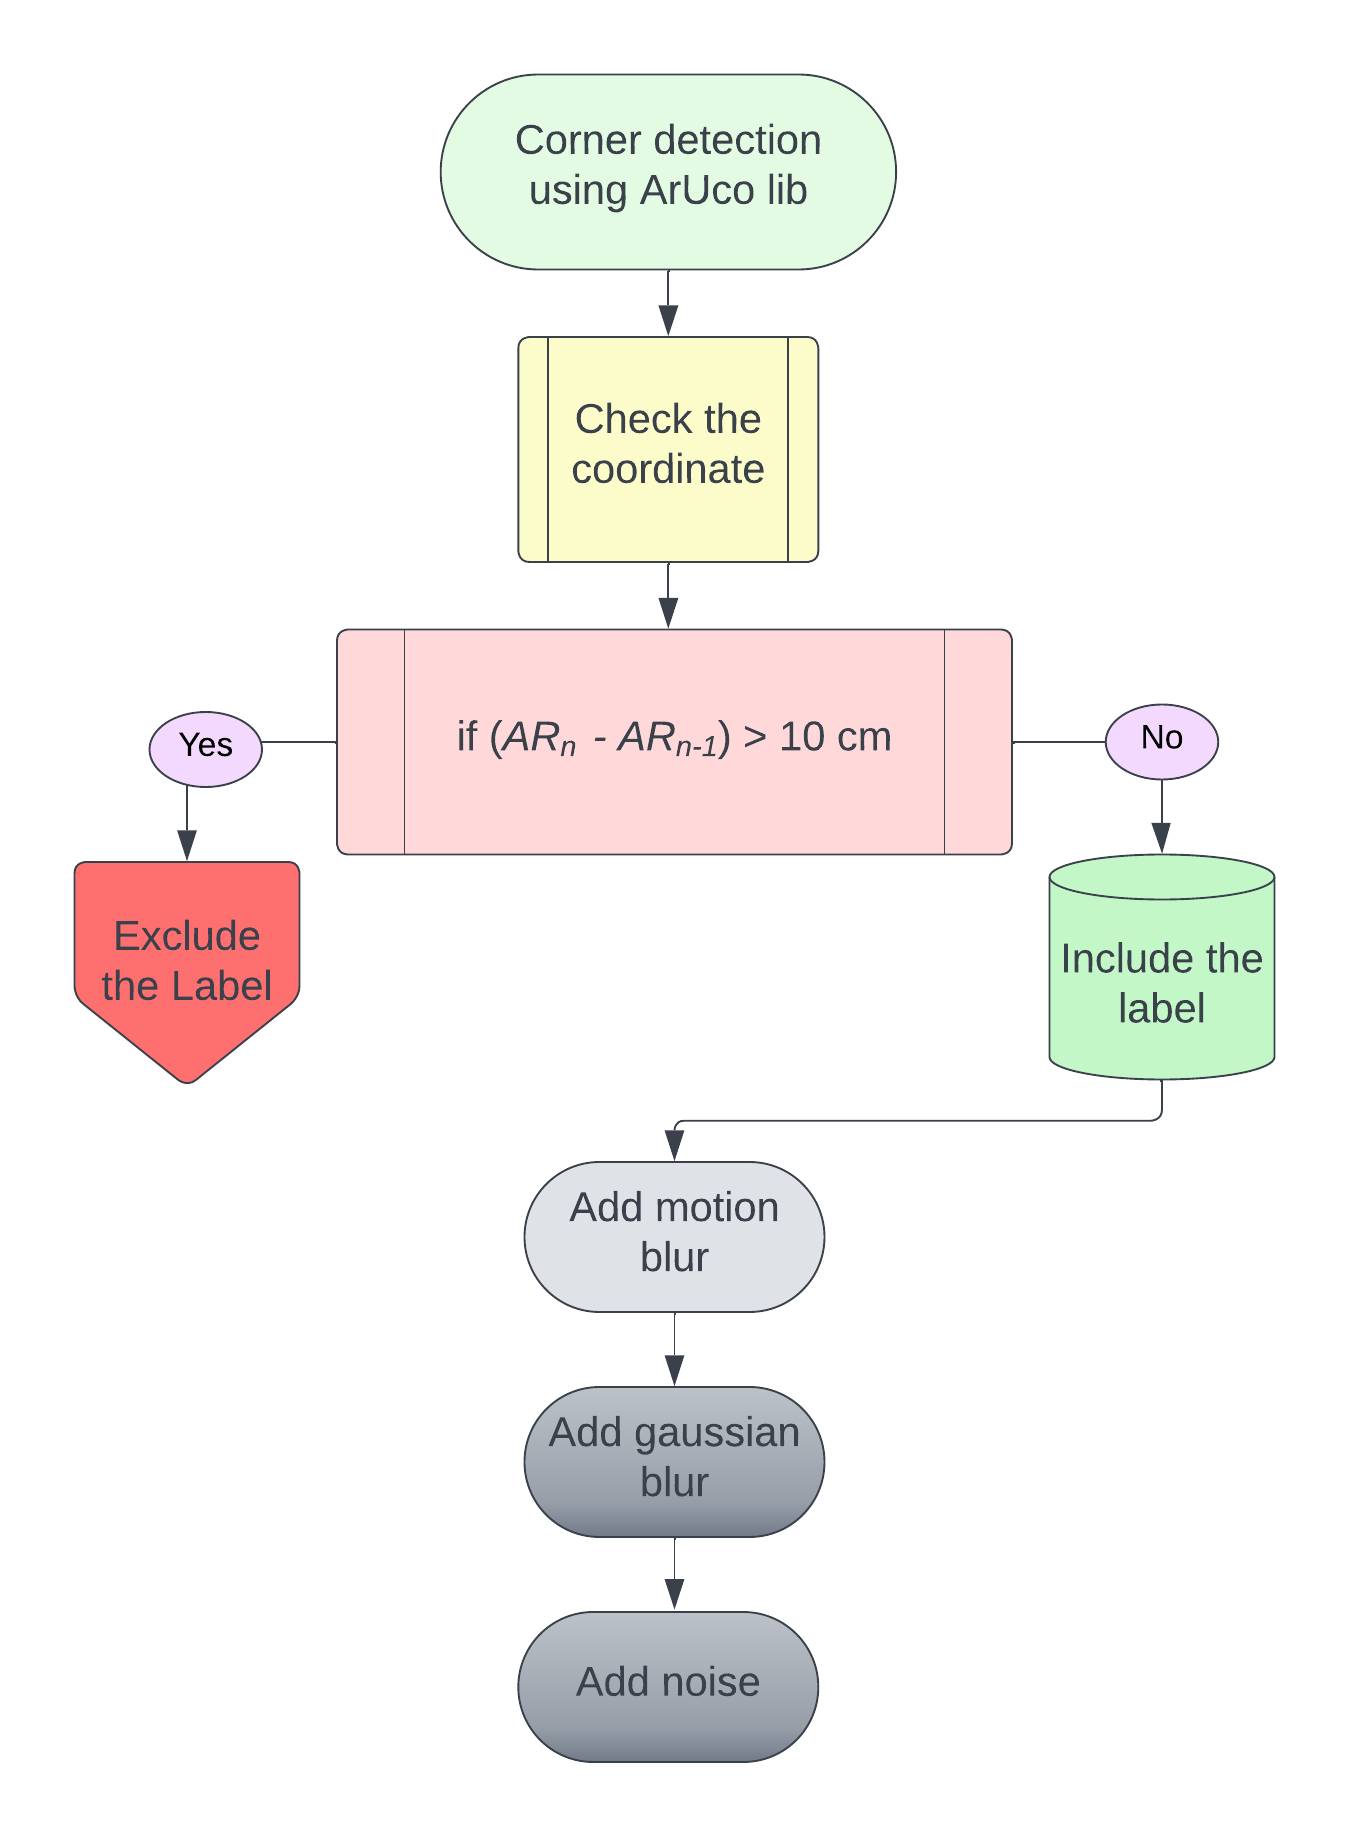
\includegraphics[width=0.6\textwidth]{m_dataset_prep.png}
    \caption{Dataset preparation flowchart}
    {algorithm for preparing the dataset, for adding different noise conditions}
    \label{fig:dataset}
\end{figure}

\begin{figure}
    \centering
    \fbox{\includegraphics[width=0.8\textwidth]{m_dataset_img.png}}
    \caption{YOLOv8 dataset, with marker labels}
    {Each tile represents an augmented frame, with different blur and intensity}
    \label{fig:dataset_img}
\end{figure}






\subsection{Training the model, and accuracy}

YOLOv8 pose model was used, speficically the \textit{YOLOv8n.pt}
with a batch size of 48, and a learning rate of 0.001. The model was trained for 200 epochs,
the training took 48 hours to complete.

Nvidia RTX 4060 laptop GPU (8GB) was used for training the model, with CPU specifications
Intel(R) Core(TM) i7-13700HX CPU @ 2.10GHz, 16.0 GB RAM.


\section{Performance of custom trained model}

\subsection{speed and detection accuracy}

The custom trained YOLOv8n model outperformed, both the ArUco standard library and DeepTag model,
specially in case of motion blur. The overall percentage of detection darastically increased.
while maintaining the pose accuracy as shown in Table \ref{tab:percentage_detection} and Table \ref{tab:pose_accuracy}.

The model inference time is shown in Fig \ref{fig:yolo_speed}, the custom trained
model can run at 33 fps, this is suitable for real-time tracking applications.
also the user can plug it with an engaging game, which does not suffer latency.

However, if the user is using a low-end GPU, the model inference time will be higher,
in our case it is around 114 fps with the RTX 4060, which is well above the 30 fps, most of the commertially
available webcamera has only 30 fps.

\begin{table}[]
    \centering
    \begin{tabular}{|lll|}
        \hline
        \multicolumn{3}{|l|}{Percentage of detection}                      \\ \hline
        \multicolumn{1}{|l|}{ArUco} & \multicolumn{1}{l|}{YOLO}  & DeepTag \\ \hline
        \multicolumn{1}{|l|}{72.8}  & \multicolumn{1}{l|}{99.76} & 44.2    \\ \hline
    \end{tabular}
    \caption{Percentage of detection}
    \label{tab:percentage_detection}

\end{table}


% Please add the following required packages to your document preamble:
% \usepackage{multirow}
\begin{table}[]
    \centering
    \begin{tabular}{|clllllllll|}
        \hline
        \multicolumn{10}{|c|}{Coordinates}                                                                                                                                                                                                                                                        \\ \hline
        \multicolumn{1}{|c|}{\multirow{2}{*}{Tag type}} & \multicolumn{3}{c|}{X cm}  & \multicolumn{3}{c|}{Y cm} & \multicolumn{3}{c|}{Z cm}                                                                                                                                                      \\ \cline{2-10}
        \multicolumn{1}{|c|}{}                          & \multicolumn{1}{l|}{Mean}  & \multicolumn{1}{l|}{STD}  & \multicolumn{1}{l|}{Mabs} & \multicolumn{1}{l|}{Mean}  & \multicolumn{1}{l|}{STD}  & \multicolumn{1}{l|}{Mabs} & \multicolumn{1}{l|}{Mean}  & \multicolumn{1}{l|}{STD}  & Mabs \\ \hline
        \multicolumn{1}{|c|}{Aruco}                     & \multicolumn{1}{l|}{-0.07} & \multicolumn{1}{l|}{0.92} & \multicolumn{1}{l|}{2.57} & \multicolumn{1}{l|}{-0.02} & \multicolumn{1}{l|}{0.10} & \multicolumn{1}{l|}{0.29} & \multicolumn{1}{l|}{-0.32} & \multicolumn{1}{l|}{1.06} & 2.61 \\ \hline
        \multicolumn{1}{|c|}{YOLO}                      & \multicolumn{1}{l|}{0.06}  & \multicolumn{1}{l|}{1.52} & \multicolumn{1}{l|}{2.91} & \multicolumn{1}{l|}{0.02}  & \multicolumn{1}{l|}{0.11} & \multicolumn{1}{l|}{0.25} & \multicolumn{1}{l|}{-0.14} & \multicolumn{1}{l|}{1.50} & 2.84 \\ \hline
        \multicolumn{1}{|c|}{Dtag}                      & \multicolumn{1}{l|}{-0.12} & \multicolumn{1}{l|}{1.57} & \multicolumn{1}{l|}{3.12} & \multicolumn{1}{l|}{0.00}  & \multicolumn{1}{l|}{0.08} & \multicolumn{1}{l|}{0.16} & \multicolumn{1}{l|}{0.84}  & \multicolumn{1}{l|}{2.99} & 6.74 \\ \hline
    \end{tabular}
    \caption{Pose accuracy of ArUco marker}
    \label{tab:pose_accuracy}

\end{table}


\begin{figure}[b!]
    \centering
    \fbox{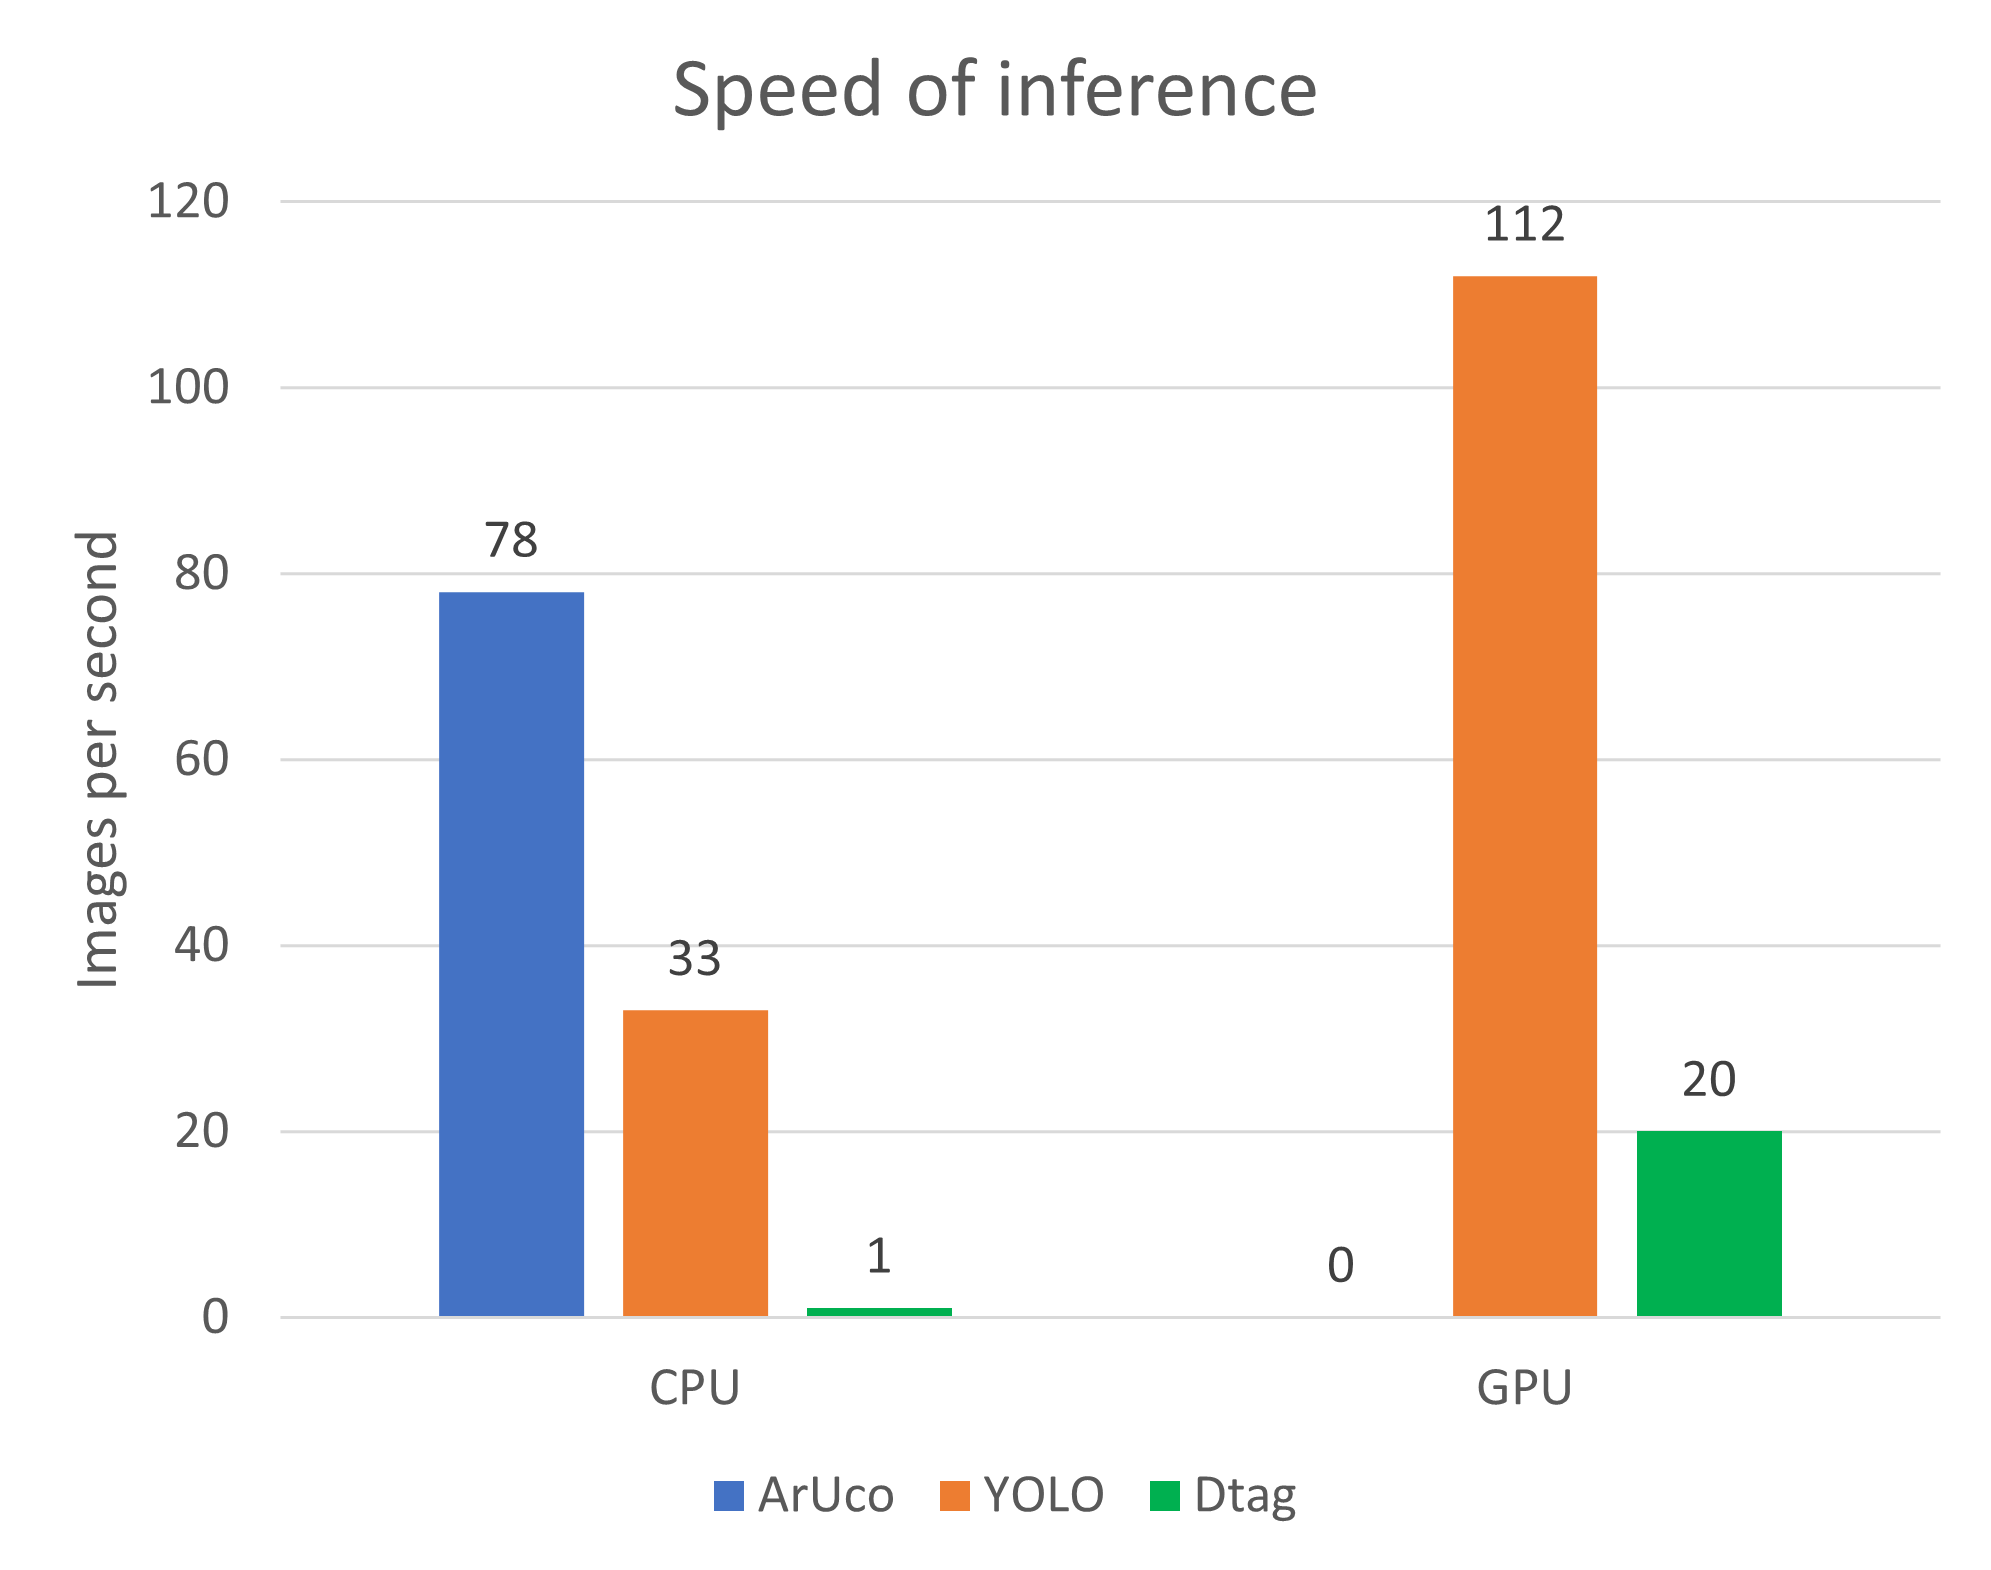
\includegraphics[width=0.8\textwidth]{m_yolo_speed.png}}
    \caption{Speed of ArUco detection using different methods}
    {a) Inference using CPU, b) Inference using GPU }
    \label{fig:yolo_speed}
\end{figure}


\chapter{Sensor-fusion based tracking}
\section{Limitations of using single ArUco marker}
As illustrated in Fig \ref{fig:occulution} a, when a user keeps the hand closer to
their trunk making the ArmBo to be at perpendicular to the field of view of the camera,
the ArUco marker will be completely occluded, and the pose estimation will be lost.

One possible way of overcoming this issue is by using multiple ArUco markers,
as shown in Fig \ref{fig:occulution} b. Two more markers are located perpendicular
to the marker $A_1$, this makes sure that the ArmBo is always in the field of view of the camera.

\begin{figure}[H]
    \centering
    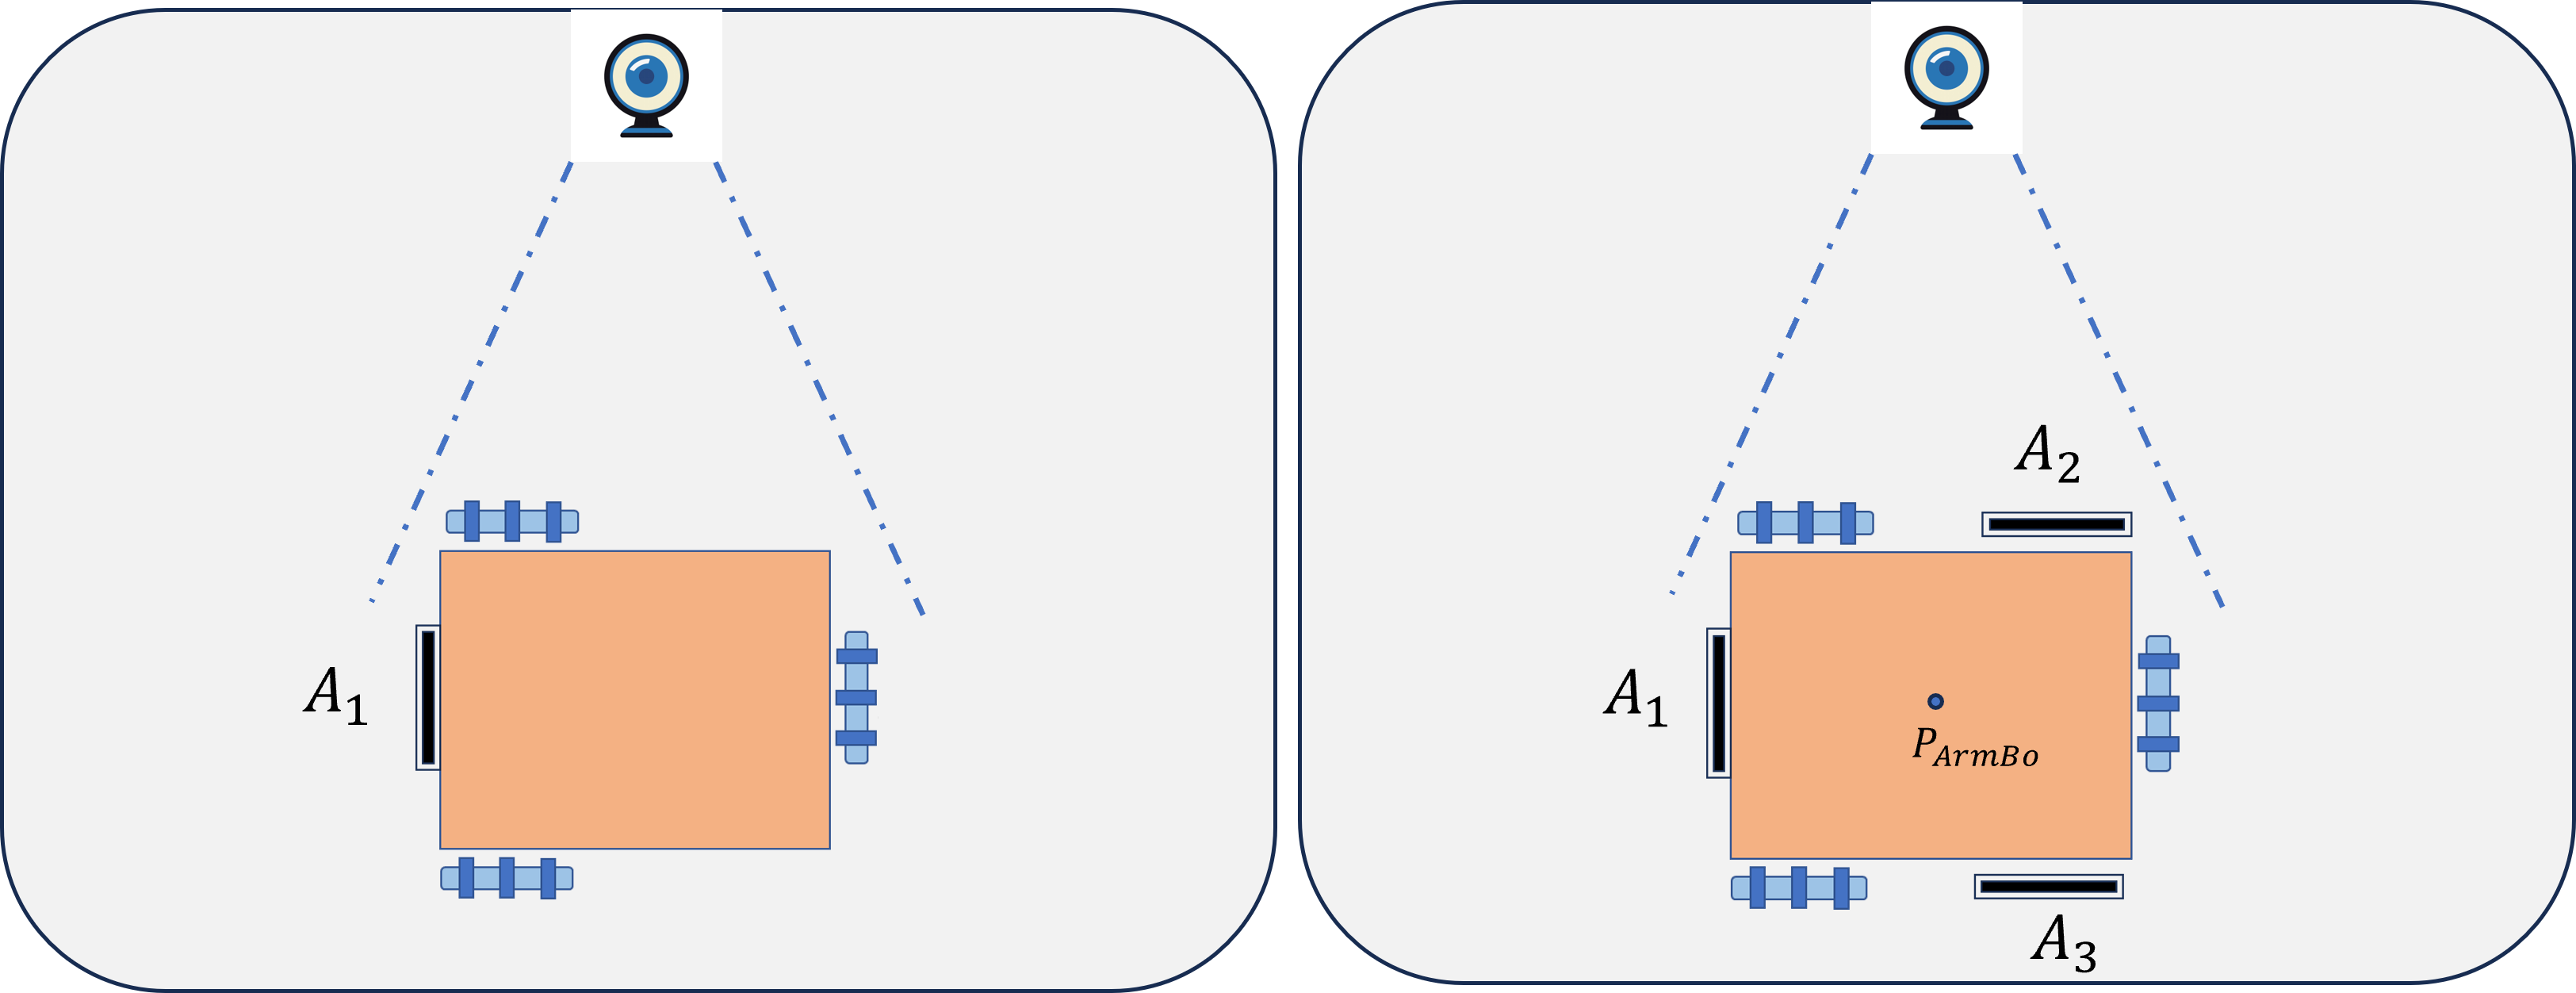
\includegraphics[width=0.9\textwidth]{m_occulution_problem.png}
    \caption{Marker occulution}
    {a) Shows the single ArUco marker being occluded from the field of view
        b) ArmBo with three ArUco marker setup, $P_{ArmBo}$ is the orgin of ArmBo}
    \label{fig:occulution}
\end{figure}

\subsection{Estimating position using three ArUco markers}
Since, we are using three markers, each marker will give us the coordinate
of the marker in the camera frame. We need to transform the coordinate of the
marker in the camera frame to the orgin of ArmBo. Then transform the coordinate
of the ArmBo to the global frame.

Here, marker $A_2$ and $A_3$ are at +90 degrees, and -90 degrees respect to the
marker $A_1$ as shown in Fig \ref{fig:occulution} b. The coordinate of the marker
$A_1$ in the camera frame is given by $P_{A_1} = (x_1, y_1, z_1)$, similarly the
coordinate of the marker $A_2$ and $A_3$ in the camera frame is given by
$P_{A_2} = (x_2, y_2, z_2)$ and $P_{A_3} = (x_3, y_3, z_3)$ respectively.

The coordinate of the ArmBo in the camera frame is given by $P_{ArmBo} = (x_{ArmBo}, y_{ArmBo}, z_{ArmBo})$.

In order to transform the coordinate of the marker $A_1, A_2, A_3$ to the ArmBo frame,
we need the current orientation of the ArmBo in the camera frame. The orientation estimation
of the ArUco marker is not accurate and has lot of noise. Thus, we use the IMU to estimate the
current orientation of the ArmBo in the camera frame.

The IMU gives us the orientation of the ArmBo in the camera frame,
which is given by $R_{ArmBo} = (r_{ArmBo}, p_{ArmBo}, y_{ArmBo})$.


\section{IMU drift correction}

Using IMU, for estimating the orientation of the ArmBo, has a major drawback,
the IMU orientation drifts over time. This is due to the accumulation of random noise
in the IMU. This can be corrected by using the ArUco marker, as the ArUco marker
gives absolute orientation but has noise when the marker is moving. However,
when the marker is stationary, the orientation of the marker is within acceptable limits.

Thus, whenever the ArmBo is stationary, the orientation of the ArUco marker is used
to correct the drift in the IMU.

\begin{figure}
    \centering
    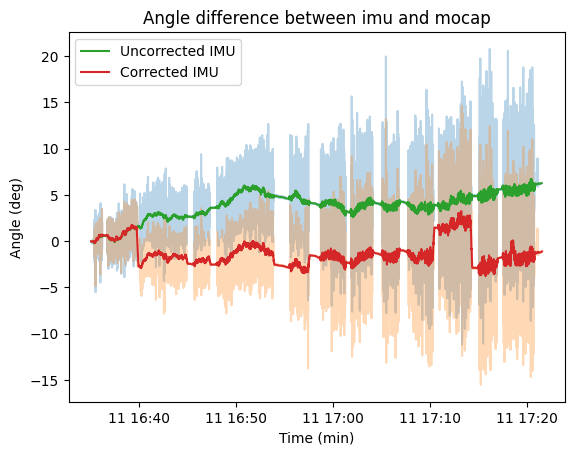
\includegraphics[width=0.9\textwidth]{m_imu_drift_correction.png}
    \caption{Correcting IMU drift using ArUco orientation}
    \label{fig:imu_correction}
\end{figure}

\section{Accuracy of three marker kinematic model}

The accuracy of the three marker kinematic model is validated by comparing the
motion capture system. The maximum error as shown in the Table \ref{tab:three_marker_accuracy}
are 4.1 cm, 0.2 cm, and 3.1 cm cm in X, Y and Z axis respectively. This is
within the acceptable limits.



\begin{table}[]
    \centering
    \begin{tabular}{|llllllllll|}
        \hline
        \multicolumn{10}{|c|}{Coordinates}                                                                                                                                                                                                                                                       \\ \hline
        \multicolumn{1}{|c|}{\multirow{2}{*}{Tag type}} & \multicolumn{3}{c|}{X cm}  & \multicolumn{3}{c|}{Y cm} & \multicolumn{3}{c|}{X cm}                                                                                                                                                     \\ \cline{2-10}
        \multicolumn{1}{|c|}{}                          & \multicolumn{1}{l|}{Mean}  & \multicolumn{1}{l|}{STD}  & \multicolumn{1}{l|}{Mabs} & \multicolumn{1}{l|}{Mean} & \multicolumn{1}{l|}{STD}  & \multicolumn{1}{l|}{Mabs} & \multicolumn{1}{l|}{Mean}  & \multicolumn{1}{l|}{STD}  & Mabs \\ \hline
        \multicolumn{1}{|l|}{YOLO WC}                   & \multicolumn{1}{l|}{-0.96} & \multicolumn{1}{l|}{2.04} & \multicolumn{1}{l|}{5.04} & \multicolumn{1}{l|}{0.09} & \multicolumn{1}{l|}{0.09} & \multicolumn{1}{l|}{0.27} & \multicolumn{1}{l|}{-0.87} & \multicolumn{1}{l|}{1.92} & 2.97 \\ \hline
        \multicolumn{1}{|l|}{YOLO WDC}                  & \multicolumn{1}{l|}{0.06}  & \multicolumn{1}{l|}{2.02} & \multicolumn{1}{l|}{4.11} & \multicolumn{1}{l|}{0.10} & \multicolumn{1}{l|}{0.09} & \multicolumn{1}{l|}{0.29} & \multicolumn{1}{l|}{-0.76} & \multicolumn{1}{l|}{1.96} & 3.16 \\ \hline
        \multicolumn{1}{|l|}{Only AR angle}             & \multicolumn{1}{l|}{-2.28} & \multicolumn{1}{l|}{2.29} & \multicolumn{1}{l|}{6.85} & \multicolumn{1}{l|}{0.08} & \multicolumn{1}{l|}{0.09} & \multicolumn{1}{l|}{0.26} & \multicolumn{1}{l|}{-0.98} & \multicolumn{1}{l|}{1.89} & 2.80 \\ \hline
    \end{tabular}
    \caption{Coordinate error}
    {YOLO WC: YOLO without drift correction, YOLO WDC: YOLO with drift correction
        Only AR angle: using the Orientation estimated by ArUco marker instead of the IMU}
    \label{tab:three_marker_accuracy}

\end{table}

\end{document}